\svnkwsave{$RepoFile: spatiotemp/chapter/reportAC.tex $}
\svnidlong {$HeadURL: svn://zero.physics.gatech.edu/siminos/spatiotemp/chapter/reportAC.tex $}
{$LastChangedDate: 2019-05-09 18:30:52 -0400 (Thu, 09 May 2019) $}
{$LastChangedRevision: 6812 $} {$LastChangedBy: predrag $}
\svnid{$Id: reportAC.tex 6812 2019-03-20 21:42:41Z predrag $}

\chapter{Andy Chen: Equilibria of KS}
% {Andy's research report}
\label{chap:reportAC}

\noindent
{\Large{\textbf{Andy Chen Fall 2017 Report}}}

\section{Introduction}
\label{sect:Repintro}
	
Here we start by studying \reqv\ solutions of the \KS\ system for $L=22$ minimal
cell\rf{SCD07,lanCvit07}, where  the dynamical system is sufficiently small
that we can think of it as a low-dimensional, or a ``few-body'' system in
Gutkin and Richter\rf{EPUR14,EDASRU14,EnUrRi15,EDUR15} condensed matter
parlance, in the limit where the columns in the Gutkin and Osipov %\rf{GutOsi15}
$2D$ symbolic dynamics spatiotemporal table
%(not a 1\dmn\ symbol sequence block), a column whose
% temporal symbolic dynamics we will know, sooner or later.
take constant values, \ie, spatial solutions are temporally steady.
Michelson\rf{Mks86} then describes the bottom row. The full Michelson \statesp\
is 4\dmn\ (3-dimensional dynamics plus a parameter), and, in addition to the
translation equivariance, it is reflection equivariant which makes it \On{2}
equivariant, so slicing together with a \Zn{2} symmetry reduction is required.

The goal of this project was to determine at least one, and hopefully a set of
{\rpo}s of the shortest periods in both the time and the space directions (with
no imposition of a fixed, finite length $L$ periodic spatial domain). However,
within the time frame of the project, I was only able to verify a Michelson
calculation of one particular \reqv\ solution, and I was not able to assign to
this solution any symbol plane, or proceed to calculation of any
spatiotemporally varying \po\ or \rpo\ solutions.


%\subsection{Overview of the project and its results}
%\label{sect:overview}
    % siminos/xiong/thesis/chapters/overview.tex
% $Author: xiong $ $Date: 2017-03-05 17:40:12 -0500 (Sun, 05 Mar 2017) $


\section{Overview of the thesis and its results}

% \PC{2017-03-01 This is my first draft. Rewrite Burak text.
%     Make this into a concise overview, like we do for our papers. State
%     clearly what is NEW that you did, in a separate paragraph
%     }
This thesis is organized as follows.
In \refchap{chap:intro}, we recall some basic facts about dissipative
dynamical systems relevant to this thesis, the traditional types of fractal
dimensions, and introduce the concept of the inertial manifold.
We review the literature on estimating
the dimension of inertial manifolds by covariant
(Lyapunov) vectors, and related algorithms.
\refchap{chap:Symmetry} is devoted to the discussion of symmetries in
dynamical systems. A reader who is familiar with the group representation
theory can skip \refsect{sect:group}.
\refsect{sec:symReduce} discusses the slicing technique we use to reduce
continuous symmetries of dynamical systems, and the tangent dynamics in the
slice.
Methods of \refchap{chap:Symmetry} are a prerequisite to the calculations of
\refchap{chap:ks}, where we study invariant structures in the
symmetry-reduced \statesp\ of the one\dmn\ \KSe.
\refChap{chap:im} contains the main result of this thesis. We investigate the
dimension of the inertial manifold in the one\dmn\ \KSe\ using the
information about the linear stability of pre/relative \po s of the system.
\refChap{chap:ped} introduces our \ped\ algorithm, essential tool for
computation of the Floquet multipliers and \Fv s reported in
\refchap{chap:im}. Readers not interested in the implementation
details can go directly to \refsect{sect:applic}, where the
performance of the algorithm is reported.
We summarize our results and outline some future directions in
\refchap{chap:conc}.

The original contributions of this thesis are mainly contained in
\refchap{chap:im} and \refchap{chap:ped}. The \ped\ introduced
in \refchap{chap:ped} is capable of resolving Floquet
multipliers as small as $10^{-27\,067}$.
In \refchap{chap:im}, we estimate the dimension of an
inertial manifold from the \po s embedded in it, and verify that our results
are consistent with earlier work based on averaging \cLvs\ over ergodic
trajectories.
This calculation is the first of its kind on this subject that is not an ergodic
average, but it actually pins down the geometry of inertial manifold's
embedding in the \statesp. It opens a door to tiling inertial manifolds by
invariant structures of system's dynamics.

%%% ======================================================================
%
%\chapter{Symmetries in dynamical systems}
%\label{chap:Symmetry}
%
%% siminos/xiong/thesis/chapters/symIntro.tex
% $Author: predrag $ $Date: 2021-06-19 11:30:00 -0400 (Sat, 19 Jun 2021) $

Symmetries play an important role in physics. In the study of
pattern formation\rf{cross93},
patterns with different symmetries form under different boundary conditions or
initial conditions. By considering symmetries only, quite a few
prototype equations such as \cGLe\rf{AKcgl02}
are proposed and have abundant applications in many fields.
So, in general,
symmetries help create a wonderful physical world for us.
However, in the analysis of chaotic systems, symmetries introduce
drifts of orbits along the symmetry directions and thus make the geometrical
structure of the global attractor more complicated than it really is.
In this case,
symmetries should be reduced before we conducting any analysis. In this chapter,
we review the basic notions of group theory, symmetry reduction
methods, and establish the relation between dynamics in the full \statesp\
and that in the symmetry-reduced \statesp.
% Finally, we factorize the
% evolution operator with respect to symmetries of the system so as to
% simplify the cycle averaging formula.

%% siminos/xiong/thesis/chapters/symGroup.tex
% $Author: predrag $ $Date: 2021-06-19 11:30:00 -0400 (Sat, 19 Jun 2021) $

\section{Group theory and symmetries: a review}
\label{sect:group}

In quantum mechanics, whenever a system exhibits some symmetry, the
corresponding symmetry group commutes with the Hamiltonian of this
system, namely, $[U(\LieEl), H] = U(\LieEl)H - HU(\LieEl) = 0$. Here
$U(\LieEl)$ denotes the operation corresponding to symmetry $g$ whose
meaning will be explained soon. The set of eigenstates with degeneracy
$\ell$, $\{\phi_1, \phi_2, \cdots, \phi_\ell\}$, corresponding to the same
system energy $H\psi_i = E_n\psi_i$, is invariant under the symmetry
since $U(\LieEl)\psi_i$ are also eigenvectors for the same energy.
This information helps us understand the spectrum of a Hamiltonian and
the quantum mechanical selection rules. We now apply the same idea to
the classical {\evOper} $\Lop^t(\ssp_e, \ssp_s)$
for a system $\flow{t}{\ssp}$ equivariant under a discrete symmetry group
$\Group=\{e, \LieEl_2, \LieEl_3,\cdots, \LieEl_{|\Group|}\}$ of order
$|\Group|$:
\begin{equation}
  \label{eq:equiva}
  \flow{t}{{D}\LieEl}\ssp)={D}(\LieEl)\,\flow{t}{\ssp} \quad \text{for}
  \quad \forall
  \LieEl\in\Group
  \,.
\end{equation}
We start with a review of some basic facts of
the group representation theory. Some examples of good references
on this topic are \refref{Hamermesh62, Tinkham}.

Suppose group $\Group$ acts on a linear space $V$ and function
$\rho(\ssp)$ is defined on this space $\ssp\in V$. Each element
$\LieEl\in\Group$ will transform point $\ssp$ to ${D}(\LieEl)\ssp$. At
the same time, $\rho(\ssp)$ is transformed to $\rho'(\ssp)$. The value
$\rho(\ssp)$ is unchanged after state point $\ssp$ is transformed to
${D}(\LieEl)\ssp$, so $\rho'({D}(\LieEl)\ssp) = \rho(\ssp)$. Denote
$U(\LieEl)\rho(\ssp)=\rho'(\ssp)$, so we have
\begin{equation}
  \label{eq:ogfx}
  U(\LieEl)\rho(\ssp) = \rho({D}(\LieEl)^{-1}\ssp)
  \,.
\end{equation}
This is how functions are transformed by group operations. Note, $D(\LieEl)$
is the representation of $G$ in the form of space transformation matrices.
The
operator $U(\LieEl)$, which acts on the function space, is not the same as
group operation ${D}(\LieEl)$, so \refeq{eq:ogfx} does not mean that
$\rho(\ssp)$ is invariant under $\Group$. \refExam{exam:C3matrRep} gives
the space transformation matrices of $\Zn{3}$.

%%%%%%%%%%%%%%%%%%%%%%%%%%%%%%%%%%%%%%%%%%%%%%%%%%%%%%%%%%%%%%%%%%%%%%
\exampl{A matrix representation of cyclic group $\Zn{3}$.}{
  \label{exam:C3matrRep}                                    \inCB
  A 3\dmn\ matrix representation of the 3-element cyclic group
  $\Zn{3}=\{e,C^{1/3},C^{2/3}\}$ is given by the three rotations by
  $2\pi/3$ around the $z$-axis in a 3\dmn\ \statesp,
  \bea
  {D}(e) &=&
  \begin{bmatrix}
    1 & & \\
    & 1 & \\
    & & 1
  \end{bmatrix}
  \,,\quad
  {D}(C^{1/3}) =
  \begin{bmatrix}
    \cos\frac{2\pi}{3}  & -\sin\frac{2\pi}{3} & \\
    \sin\frac{2\pi}{3}  & ~\cos\frac{2\pi}{3}  & \\
    & & 1
  \end{bmatrix}
  \,,
  \continue
  {D}(C^{2/3}) &=&
  \begin{bmatrix}
    \cos\frac{4\pi}{3}  & -\sin\frac{4\pi}{3}  & \\
    \sin\frac{4\pi}{3}  & ~\cos\frac{4\pi}{3}  & \\
    & & 1
  \end{bmatrix}
  \,.
  \nnu
  \eea
  %\index{matrix rep!cyclic group}
  ~~(continued in \refexam{exam:C3regularRep})
}
%%%%%%%%%%%%%%%%%%%%%%%%%%%%%%%%%%%%%%%%%%%%%%%%%%%%%%%%%%%%%%%%%%%%%%

\subsection{Regular representation}
An operator $U(\LieEl)$ which acts on an infinite\dmn\ function space
is too abstract to analyze.
We would like to represent it in a more familiar way.
Suppose there is a function $\rho(\ssp)$ with symmetry $\Group$ defined in full
\statesp\ $\pS$, then full \statesp\ can be decomposed as a union
of $|\Group|$ tiles each of which is obtained by transforming the fundamental
domain,
\begin{equation}
  \label{eq:domain}
  \pS =  \bigcup_{g\in \Group}g\pSRed
  \,,
\end{equation}
where $\pSRed$ is the chosen fundamental domain.
So $\rho(\ssp)$ takes $|G|$ different forms by \refeq{eq:ogfx} in each sub-domain
in \refeq{eq:domain}. Now, we obtained a natural choice of a set of bases in this
function space called the \emph{regular bases},
\beq
\label{eq:RegBasis}
\{ \rho_1^{reg}(\sspRed), \rho_2^{reg}(\sspRed), %\rho_3^{reg}(\sspRed),
\cdots, \rho_{|\Group|}^{reg}(\sspRed)\}
=
\{
\rho(\sspRed), \rho(\LieEl_2\sspRed), % \rho(\LieEl_3\sspRed),
\cdots, \rho(\LieEl_{|\Group|}\sspRed) \}
\,.
\eeq
Here, for notation simplicity we use
$\rho(\LieEl_i\sspRed)$ to represent $\rho(D(\LieEl_i\sspRed))$ without
ambiguity.
These bases are
constructed by applying $U(\LieEl^{-1})$ to $\rho(\sspRed)$ for each
$\LieEl\in\Group$, with $\sspRed$ a point in the fundamental domain.
The [$|G|\!\times\!|G|$] matrix representation of the
action of $U(\LieEl)$ in bases \refeq{eq:RegBasis} is called the \emph{(left)
regular representation} $D^{reg}(\LieEl)$. Relation \refeq{eq:ogfx} says that
$D^{reg}(\LieEl)$ is a permutation matrix, so each row or column has only one nonzero
element.

We have a simple trick to obtain the regular representation quickly.
Suppose the element at the $i$th row and
the $j$th column of $D^{reg}(\LieEl)$
is $1$. It means
$\rho(\LieEl_i\sspRed) = U(\LieEl) \rho(\LieEl_j\sspRed)$, which
is $g_i=\LieEl^{-1}g_j \implies g^{-1} = g_i g_j^{-1}$. Namely,
\beq
D^{reg}(\LieEl)_{ij} = \delta_{\LieEl^{-1},\, g_i g_j^{-1}}
\,.
\ee{eq:RegRep}
So if we arrange the
columns of the multiplication table by the inverse of the group elements,
then setting positions with $\LieEl^{-1}$ to 1 defines the regular
representation $D^{reg}(\LieEl)$. Note, the above relation can
be further simplified to $g = g_jg_i^{-1}$, but it exchanges the rows and
columns of the multiplication table, so $g = g_jg_i^{-1}$
should not be used to get $D^{reg}(\LieEl)$.
On the other hand, it is easy to see
that the regular representation of group element $e$ is always the identity matrix.

%%%%%%%%%%%%%%%%%%%%%%%%%%%%%%%%%%%%%%%%%%%%%%%%%%%%%%%%%%%%%%%%%%%%%%%
\begin{table}[h]
  \caption[ The multiplication tables of the $\Zn{2}$ and $\Zn{3}$]{
    The multiplication tables of the (a) group $\Zn{2}$ and (b) $\Zn{3}$.
  }
  \label{tab:C3MultTab}
  \begin{center}
    \centering
    (a)
    \begin{tabular}{c | c c}
      $\Zn{2}$         & $e$        & $\sigma^{-1}$  \\ \hline
      $e$              & $e$        & $\sigma$   \\
      $\sigma$ & $\sigma$  & $e$         \\
    \end{tabular}
    \quad
    (b)
    \begin{tabular}{c | c c c}
      $\Zn{3}$         & $e$        & $(C^{1/3})^{-1}$ & $(C^{2/3})^{-1}$ \\ \hline
      $e$              & $e$        & $C^{2/3}$ & $C^{1/3}$  \\
      $C^{1/3}$ & $C^{1/3}$  & $e$       & $C^{2/3}$   \\
      $C^{2/3}$ & $C^{2/3}$  & $C^{1/3}$ & $e$
    \end{tabular}
  \end{center}
\end{table}
%%%%%%%%%%%%%%%%%%%%%%%%%%%%%%%%%%%%%%%%%%%%%%%%%%%%%%%%%%%%%%%%%%%%%%%


%%%%%%%%%%%%%%%%%%%%%%%%%%%%%%%%%%%%%%%%%%%%%%%%%%%%%%%%%%%%%%%%%%%%%%
\exampl{The regular representation of cyclic group $\Zn{3}$.}{
  \label{exam:C3regularRep}                                    \inCB
  (continued from \refexam{exam:C3matrRep})~~
  Take an arbitrary function $\rho(\ssp)$ over the \statesp\ $\ssp \in \pS$, and
  define a fundamental domain $\pSRed$ as a 1/3 wedge, with axis $z$ as its
  (symmetry invariant) edge. The \statesp\ is tiled with three copies of the wedge,
  \[
    \pS =  \pSRed_1\cup\pSRed_2\cup\pSRed_3
    =  \pSRed\cup C^{1/3}\pSRed\cup C^{2/3}\pSRed
    \,.
  \]
  Function $\rho(\ssp)$ can be written as the 3\dmn\ vector of functions
  over the fundamental domain $\sspRed \in \pSRed$,
  \beq
  (\rho_1^{reg}(\sspRed),\rho_2^{reg}(\sspRed),\rho_3^{reg}(\sspRed))
  = (\rho(\sspRed),\rho(C^{1/3}\sspRed),\rho(C^{2/3}\sspRed))
  \,.
  \ee{eq:C3RegRep}
  The multiplication table of $\Zn{3}$ is given in \reftab{tab:C3MultTab}.
  By \refeq{eq:RegRep}, the regular representation matrices
  $D^{reg}(\LieEl)$ have `1' at the location of $\LieEl^{-1}$ in the
  multiplication table, `0' elsewhere. The actions of the operator
  $U(\LieEl)$ are now represented by permutations matrices (blank entries
  are zeros):
  \beq
  D^{reg}(e) = %&=&
  \begin{bmatrix}
    1 & & \\
    & 1 & \\
    & & 1 \\
  \end{bmatrix} \,,  \quad
  % \continue
  D^{reg}(C^{1/3}) = %&=&
  \begin{bmatrix}
    ~ & 1 & ~\\
    ~ & ~ & 1\\
    1 & ~ & ~ \\
  \end{bmatrix}\,,  \quad
  D^{reg}(C^{2/3}) =
  \begin{bmatrix}
    ~ & ~ & 1\\
    1 & ~ & ~\\
    ~ & 1 & ~ \\
  \end{bmatrix}
  \,.
  \label{eq:C3reg}
  \eeq
  %\index{regular rep!cyclic group}
} %end \exampl{A regular representation of cyclic group $\Zn{3}$.}{
%%%%%%%%%%%%%%%%%%%%%%%%%%%%%%%%%%%%%%%%%%%%%%%%%%%%%%%%%%%%%%%%%%%%%%

%%%%%%%%%%%%%%%%%%%%%%%%%%%%%%%%%%%%%%%%%%%%%%%%%%%%%%%%%%%%%%%%%%%%%%%
\begin{table}[h]
  \caption[The multiplication table of  $\Dn{3}$]{
    The multiplication table of  $\Dn{3}$, the group of symmetries of an equilateral
    triangle.
  }
  \label{tab:D3MultTab}
  \begin{center}
    \centering
    \begin{tabular}{c | c c c c c c}
      $D_3$ & $e$ & $(\sigma_{12})^{-1}$ & $(\sigma_{23})^{-1}$ & $(\sigma_{31})^{-1}$
      & $(C^{1/3})^{-1}$ & $(C^{2/3})^{-1}$ \\ \hline
      $e$ & $e$ & $\sigma_{12}$ & $\sigma_{23}$ & $\sigma_{31}$  & $C^{2/3}$ & $C^{1/3}$\\
      $\sigma_{12}$ & $\sigma_{12}$ & $e$ & $C^{1/3}$ & $C^{2/3}$  & $\sigma_{31}$ & $\sigma_{23}$\\
      $\sigma_{23}$ & $\sigma_{23}$ & $C^{2/3}$ & $e$ & $C^{1/3}$  & $\sigma_{12}$ & $\sigma_{31}$\\
      $\sigma_{31}$ & $\sigma_{31}$ & $C^{1/3}$ & $C^{2/3}$ & $e$  & $\sigma_{23}$ & $\sigma_{12}$\\
      $C^{1/3}$ & $C^{1/3}$ & $\sigma_{31}$ & $\sigma_{12}$ & $\sigma_{23}$ & $e$ & $C^{2/3}$   \\
      $C^{2/3}$ & $C^{2/3}$ & $\sigma_{23}$ & $\sigma_{31}$ & $\sigma_{12}$ & $C^{1/3}$ & $e$
    \end{tabular}
  \end{center}
\end{table}
%%%%%%%%%%%%%%%%%%%%%%%%%%%%%%%%%%%%%%%%%%%%%%%%%%%%%%%%%%%%%%%%%%%%%%%

%%%%%%%%%%%%%%%%%%%%%%%%%%%%%%%%%%%%%%%%%%%%%%%%%%%%%%%%%%%%%%%%%%%%%%
\exampl{The regular representation of dihedral group $\Dn{3}$.}{
  \label{exam:D3regularRep}                                    \inCB
  $\Dn{3} = \{ e, \sigma_{12}, \sigma_{23}, \sigma_{31}, C^{1/3}, C^{2/3}\}$
  represents the symmetries of a triangle with equal sides.
  $C^{1/3}$ and  $C^{2/3}$ are rotations by $2\pi/3$ and $4\pi/3$ respectively.
  $\sigma_{12}, \sigma_{23}$ and $\sigma_{31}$ are 3 reflections.
  The regular bases in this case are
  \[
    \left(\rho(\sspRed),\,\rho(\sigma_{12}\sspRed) ,\, \rho(\sigma_{23}\sspRed) ,\,
      \rho(\sigma_{31}\sspRed) ,\, \rho(C^{1/3}\sspRed) ,\, \rho(C^{2/3}\sspRed)\right)
    \,.
  \]
  It helps us obtain the multiplication table quickly by the following relations
  \begin{equation}
    \label{eq:C3relations}
    \sigma_{31} = C^{1/3}\sigma_{12} \,,\quad
    \sigma_{23} = C^{2/3}\sigma_{12}\,,\quad
    C^{1/3}\sigma_{12} = \sigma_{12}C^{2/3} \,,\quad
    C^{2/3}\sigma_{12} = \sigma_{12}C^{1/3}
    \,.
  \end{equation}
  The multiplication table of
  $\Dn{3}$ % = \{ e, \sigma_{12}, \sigma_{23}, \sigma_{31}, C^{1/3}, C^{2/3}\}$
  is given in \reftab{tab:D3MultTab}.
  By \refeq{eq:RegRep}, the 6 regular representation matrices
  $D^{reg}(\LieEl)$ have `1' at the location of $\LieEl^{-1}$
  in the multiplication table, `0' elsewhere.
  For example, the regular representation of the action of
  operators $U(\sigma_{23})$ and
  $U(C^{2/3})$ are, respectively:
  \[
    D^{reg}(\sigma_{23}) =
    \begin{bmatrix}
      0 & 0 & 1 & 0 & 0 & 0 \\
      0 & 0 & 0 & 0 & 0 & 1 \\
      1 & 0 & 0 & 0 & 0 & 0 \\
      0 & 0 & 0 & 0 & 1 & 0 \\
      0 & 0 & 0 & 1 & 0 & 0 \\
      0 & 1 & 0 & 0 & 0 & 0
    \end{bmatrix}
    \,,\quad
    D^{reg}(C^{1/3}) =
    \begin{bmatrix}
      0 & 0 & 0 & 0 & 1 & 0 \\
      0 & 0 & 0 & 1 & 0 & 0 \\
      0 & 1 & 0 & 0 & 0 & 0 \\
      0 & 0 & 1 & 0 & 0 & 0 \\
      0 & 0 & 0 & 0 & 0 & 1 \\
      1 & 0 & 0 & 0 & 0 & 0
    \end{bmatrix}
    \,.
  \]
  %%%%%%%%%%%%%%%%%%%%%%%%%%%%%%%%%%%%%%%%%%%%%%%%%%%%%%%%%%%%%%%%%%%%%%
} %end \exampl{The regular representation of dihedral group $\Dn{3}$.}{

\subsection{Irreducible representations}

$U(\LieEl)$ is a linear operator under the regular bases.
Any linearly independent combination of the regular bases can be used as
new bases, and then the representation of $U(\LieEl)$ changes respectively.
So we ask a question: can we find a new set of bases
\begin{equation}
  \rho^{irr}_i=\sum_j S_{ij}\rho^{reg}_j
  \label{eq:trans}
\end{equation}
such that the new representation $D^{irr}(\LieEl) = SD^{reg}(\LieEl)S^{-1}$ is block-diagonal
for any $\LieEl\in\Group$ ?
\begin{equation}
  D^{irr}(\LieEl) =
  \begin{bmatrix}
    D^{(1)}(\LieEl) & & \\
    & D^{(2)}(\LieEl) & \\
    & & \ddots \\
  \end{bmatrix}
  = \bigoplus_{\mu=1}^{r} d_\mu D^{(\mu)}(\LieEl)
  \,.
  \label{eq:irre}
\end{equation}
In such a block-diagonal representation, the
subspace corresponding to each diagonal block is invariant under $\Group$
and the action of $U(\LieEl)$ can be analyzed subspace by subspace.
It can be easily checked that for each $\mu$, $D^{(\mu)}(\LieEl)$ for all
$\LieEl\in\Group$ form another representation (\emph{irreducible
  representation}, or \emph{irrep}) of group $\Group$.
Here, $r$ denotes the total number of
irreps of $\Group$. The same irrep may show up more than once in the decomposition
\refeq{eq:irre}, so the coefficient $d_{\mu}$ denotes the number of its
copies.  Moreover, it is proved\rf{Hamermesh62} that $d_{\mu}$ is also equal to the dimension
of $D^{(\mu)}(\LieEl)$ in \refeq{eq:irre}.
Therefore, we have a relation
\[
  \sum_{\mu=1}^r d_\mu^2 = |G|
  \,.
\]

%%%%%%%%%%%%%%%%%%%%%%%%%%%%%%%%%%%%%%%%%%%%%%%%%%%%%%%%%%%%%%%%%%%%%%
\exampl{Irreps of cyclic group $\Zn{3}$.}{
  \label{exam:C3irReps}                                     \inCB
  (continued from \refexam{exam:C3regularRep})~~
  For $\Zn{2}$ whose multiplication table is in \reftab{tab:C3MultTab}, we can form
  the symmetric base $\rho(\sspRed) + \rho(\sigma\sspRed)$
  and the antisymmetric base $\rho(\sspRed) - \rho(\sigma\sspRed)$. You can verify
  that under these new bases, $\Zn{2}$ is block-diagonalized.
  We would like to generalize this symmetric-antisymmetric
  decomposition to the order 3 group $\Zn{3}$. Symmetrization
  can be carried out on any number of functions, but there is no obvious
  anti-symmetrization. We draw instead inspiration from the Fourier
  transformation for a finite periodic lattice, and construct from the
  regular bases \refeq{eq:C3RegRep} a new set of bases
  \bea
  \rho^{irr}_0(\sspRed) &=& \frac{1}{3}\left[
    \rho(\sspRed) ~+~ \rho(C^{1/3} \sspRed) ~+~ \rho(C^{2/3} \sspRed)
  \right]
  \label{eq:c3f1}\\
  \rho_1^{irr}(\sspRed) &=& \frac{1}{3}\left[
    \rho(\sspRed) + \omega\,\rho(C^{1/3} \sspRed) + \omega^2 \rho(C^{2/3} \sspRed)
  \right]
  \label{eq:c3f2}\\
  \rho_2^{irr}(\sspRed) &=& \frac{1}{3}\left[
    \rho(\sspRed) + \omega^2 \rho(C^{1/3} \sspRed) + \omega\,\rho(C^{2/3} \sspRed)
  \right]
  \label{eq:c3f2}
  \,.
  \eea
  Here $\omega = e^{2i\pi/3}$.
  The representation of group $\Zn{3}$ in this new bases is block-diagonal
  by inspection:
  \begin{equation}
    D^{irr}(e) =
    \begin{bmatrix}
      1 & & \\
      & 1 & \\
      & & 1 \\
    \end{bmatrix} \,,\quad
    D^{irr}(C^{1/3}) =
    \begin{bmatrix}
      1 & 0 & 0\\
      0 & \omega & 0\\
      0 & 0 & \omega^2 \\
    \end{bmatrix}  \,,\quad
    D^{irr}(C^{2/3}) =
    \begin{bmatrix}
      1 & 0 & 0\\
      0 & \omega^2 & 0\\
      0 & 0 & \omega \\
    \end{bmatrix}
    \,.
    \label{eq:c3irr}
  \end{equation}
  So $\Zn{3}$ has three 1\dmn\ irreps. Generalization to any
  $\Zn{n}$ is immediate: this is just a finite lattice Fourier transform.
}% end \exampl{Irreps of cyclic group $\Zn{3}$
%%%%%%%%%%%%%%%%%%%%%%%%%%%%%%%%%%%%%%%%%%%%%%%%%%%%%%%%%%%%%%%%%%%%%%

\paragraph{Character tables.}
Finding a transformation $S$ which simultaneously block-diagonalizes the
regular representation of each group element sounds difficult.
However, suppose it can be achieved and we obtain a set of irreps $D^{(\mu)}(\LieEl)$,
then according to Schur's lemmas\rf{Hamermesh62}, $D^{(\mu)}(\LieEl)$ must satisfy a set of
orthogonality relations:
\begin{equation}
  \label{eq:ortho}
  \frac{d_\mu}{|G|} \sum_g D_{il}^{(\mu)}(\LieEl) D_{mj}^{(\nu)}(g^{-1}) = \delta_{\mu \nu}
  \delta_{ij} \delta_{lm}
  \,.
\end{equation}
Denote the trace of irrep $D^{(\mu)}$ as $\chi^{(\mu)}$, which is referred to as
the \emph{character} of $D^{(\mu)}$. Properties of irreps can be derived from
\refeq{eq:ortho}, and we list them as follows:
\begin{enumerate}
\item The number of irreps is the same as the number of
  classes.
\item Dimensions of irreps satisfy
  $\sum_{\mu=1}^{r} d^2_\mu = |G| $
\item Orthonormal relation I :
  $\sum_{i=1}^{r} |K_i| \chi_i^{(\mu)} \chi_i^{(\nu)*} = |G|\delta_{\mu \nu} $. \\
  Here, the summation goes through all classes of this group, and $|K_i|$ is
  the number of elements in class $i$. This weight comes from the fact that
  elements in the same class have the same character. Symbol $*$ means
  the complex conjugate.
\item Orthonormal relation II :
  $\sum_{\mu=1}^{r} \chi_i^{(\mu)} \chi_j^{(\mu)*} = \frac{|G|}{|K_i|}\delta_{ij} $. \\
\end{enumerate}
The characters for all classes and irreps of a finite group are
conventionally arranged into a \emph{character table}, a square matrix
whose rows represent different
classes and columns represent different irreps.
Rules 1 and 2 help determine the number of irreps and
their dimensions. As the matrix representation of class $\{e\}$ is always the
identity matrix, the first row is always the dimension of the
corresponding representation. All entries of the first column are always 1,
because the symmetric irrep is always one\dmn. To compute the
remaining entries, we should use properties 3, 4 and the class multiplication
tables.   Spectroscopists conventions use labels $A$ and $B$ for
symmetric, respectively antisymmetric nondegenerate irreps, and
$E$, $T$, $G$, $H$ for doubly, triply, quadruply, quintuply degenerate irreps.

%%%%%%%%%%%%%%%%%%%%%%%%%%%%%%%%%%%%%%%%%%%%%%%%%%%%%%%%%%%%%%%%%%%%%%
\begin{table}[h]
  \caption[Character tables of $\Zn{2}$, $\Zn{3}$ and $\Dn{3}$]{
    Character tables of $\Zn{2}$, $\Zn{3}$ and $\Dn{3}$.
    The classes
    $\{\sigma_{12},\sigma_{13},\sigma_{14}\}$, $\{ C^{1/3}, C^{2/3} \}$
    are denoted $3\sigma$, $2C$, respectively.
  }
  \label{tab:D3charac}
  \centering
  \begin{tabular}{c|ccc}
    $\Zn{2}$ & $A$ & $B$ \\
    \hline
    $e$  & 1 & 1  \\
    $\sigma$ & 1 & -1
  \end{tabular}
  \qquad
  \begin{tabular}{c|ccc}
    $\Zn{3}$ & $A$ & \multicolumn{2}{c}{$E$}  \\
    \hline
    $e$ & 1 & 1  & 1 \\
    $C^{1/3}$ & 1 & $\omega$ & $\omega^2$ \\
    $C^{2/3}$ & 1 & $\omega^2$  & $\omega$
  \end{tabular}
  \qquad
  \begin{tabular}{c|ccc}
    $\Dn{3}$ & $A$ & $B$ & $E$ \\
    \hline
    $e$ & 1 & 1  & 2 \\
    $3\sigma$ & 1 & -1 & 0 \\
    $2C$   & 1 & 1  & -1
  \end{tabular}
\end{table}
%%%%%%%%%%%%%%%%%%%%%%%%%%%%%%%%%%%%%%%%%%%%%%%%%%%%%%%%%%%%%%%%%%%%%%

%%%%%%%%%%%%%%%%%%%%%%%%%%%%%%%%%%%%%%%%%%%%%%%%%%%%%%%%%%%%%%%%%%%%%%
\exampl{Character table of $\Dn{3}$.}{\label{exam:D3charTab}         \inCB
  (continued from \refexam{exam:D3regularRep})~~
  Let us construct \reftab{tab:D3charac}.
  one\dmn\ representations are denoted by $A$ and $B$, depending on
  whether the basis function is symmetric or antisymmetric with respect to
  transpositions $\sigma_{ij}$. $E$ denotes the two\dmn\ representation.
  As
  $\Dn{3}$ has 3 classes, the dimension sum rule $d_1^2+d_2^2+d_3^2 = 6$
  has only one solution $d_1=d_2=1$, $d_3=2$. Hence there are two one\dmn\
  irreps and one two\dmn\ irrep. The first row is $1,1,2$, and the first
  column is $1,1,1$ corresponding to the one\dmn\ symmetric representation. We take
  two approaches to figure out the remaining 4 entries. First, since $B$
  is an antisymmetric one\dmn\ representation, so the characters should be $\pm 1$.
  We anticipate $\chi^{B}(\sigma) = -1$ and can quickly figure out the
  remaining 3 positions. Then we check that the obtained table satisfies the
  orthonormal relations. Second, denote $\chi^{B}(\sigma)=x$ and
  $\chi^E(\sigma)=y$, then from the orthonormal relation of the second
  column with the first column and itself, we obtain $1+x+2y=0$ and
  $1+x^2+y^2=6/3$. Then we get two sets of solutions, one of which is
  incompatible with other orthonormal relations, so we are left with
  $x=-1$, $y=0$.
  Similarly, we can get the other two characters.
} %end \exampl{Character table of $\Dn{3}$.}{\label{exam:D3charTab}
%%%%%%%%%%%%%%%%%%%%%%%%%%%%%%%%%%%%%%%%%%%%%%%%%%%%%%%%%%%%%%%%%%%%%%

\subsection{Projection operator}
We have listed the properties of irreps and the
techniques of constructing a character table, but we still do not know how to
construct the similarity transformation $S$ which takes a regular representation into a
block-diagonal form. Think of it in another way,
each irrep is associated with an invariant subspace, so by
projecting an arbitrary function $\rho(\ssp)$ into its invariant subspaces, we
find the transformation \refeq{eq:trans}.
One of these invariant subspaces is $\sum_g \rho(g\sspRed)$, which is the basis of
the one\dmn\ symmetric irrep $A$. For $\Zn{3}$, it is \refeq{eq:c3f1}.
But how to get the others? We resort to the projection operator:
\begin{equation}
  \label{eq:projecIrre}
  P^{(\mu)}_{i} = \frac{d_\mu}{|G|}\sum_g \left(D^{(\mu)}_{ii} (\LieEl)\right)^* U(g)
  \,.
\end{equation}
It projects an arbitrary function into the $i$th basis of irrep
$D^{(\mu)}$ provided the diagonal elements of this representation
$D^{(\mu)}_{ii}$ are known. $ P^{(\mu)}_{i} \rho(\ssp) = \rho^{(\mu)}_i$.
Here, symbol $*$ means the complex conjugate. For unitary groups
$\left(D^{(\mu)}_{ii} (\LieEl)\right)^* = D^{(\mu)}_{ii} (\LieEl^{-1})$.
Summing $i$ in \refeq{eq:projecIrre} gives
\begin{equation}
  \label{eq:projectSum}
  P^{(\mu)} = \frac{d_\mu}{|G|}\sum_g \left(\chi^{(\mu)}(\LieEl)\right)^*U(g)
  \,.
\end{equation}
This is also a projection operator which projects an arbitrary function onto
the sum of the bases of irrep $D^{(\mu)}$.

Note, for one\dmn\ representations, \refeq{eq:projectSum}
is equivalent to \refeq{eq:projecIrre}. The projection operator is
known after we obtain
the character table, since the character of an one\dmn\ matrix is the matrix itself.
However, for two\dmn\ or higher\dmn\ representations, we need to know the
diagonal elements $D^{(\mu)}_{ii}$ in order to get the bases of invariant subspaces. That is to say,
\refeq{eq:projecIrre} should be used instead of \refeq{eq:projectSum} in this case.
\refExam{exam:D3irrepBases} illustrates this point. The two one\dmn\ irreps are obtained
by \refeq{eq:projectSum}, but the other four two\dmn\ irreps are obtained by
\refeq{eq:projecIrre}.

%%%%%%%%%%%%%%%%%%%%%%%%%%%%%%%%%%%%%%%%%%%%%%%%%%%%%%%%%%%%%%%%%%%%%%
\exampl{Bases for irreps of $\Dn{3}$.}{
  \label{exam:D3irrepBases}                                       \inCB
  (continued from \refexam{exam:D3regularRep})~~
  We use projection operator \refeq{eq:projectSum} to obtain the
  bases of irreps of $\Dn{3}$.
  From \reftab{tab:D3charac}, we have
  \begin{align}
    P^{A}\rho(\sspRed)
    & = \frac{1}{6}
      \left[
      \rho(\sspRed) + \rho(\sigma_{12}\sspRed) + \rho(\sigma_{23}\sspRed)
      + \rho(\sigma_{31}\sspRed) + \rho(C^{1/3} \sspRed) + \rho(C^{2/3} \sspRed)
      \right] \\
    P^{B}\rho(\sspRed)
    & = \frac{1}{6}
      \left[
      \rho(\sspRed) - \rho(\sigma_{12}\sspRed) - \rho(\sigma_{23}\sspRed)
      - \rho(\sigma_{31}\sspRed) + \rho(C^{1/3} \sspRed) + \rho(C^{2/3} \sspRed)
      \right]
      \,.
  \end{align}
  For projection into irrep E, we need to figure out the explicit
  matrix representation first. Obviously, the following 2 by 2 matrices are E irreps.
  \begin{equation}
    D^E(e) =
    \begin{bmatrix}
      1 & 0\\
      0 & 1 \\
    \end{bmatrix} \,,\quad
    D^E(C^{1/3}) =
    \begin{bmatrix}
      \omega & 0 \\
      0 & \omega^2 \\
    \end{bmatrix}  \,,\quad
    D^E(C^{2/3}) =
    \begin{bmatrix}
      \omega^2 & 0 \\
      0 & \omega \\
    \end{bmatrix}  \,
    \label{eq:c3E_1}
  \end{equation}
  \begin{equation}
    D^E(\sigma_{12}) =
    \begin{bmatrix}
      0 & 1 \\
      1 & 0\\
    \end{bmatrix} \,,\quad
    D^E(\sigma_{23}) =
    \begin{bmatrix}
      0 & \omega^2 \\
      \omega & 0 \\
    \end{bmatrix}  \,,\quad
    D^E(\sigma_{31}) =
    \begin{bmatrix}
      0 & \omega  \\
      \omega^2 & 0 \\
    \end{bmatrix}  \,.
    \label{eq:c3E_2}
  \end{equation}
  So apply projection operator \refeq{eq:projecIrre} on $\rho(\sspRed)$ and
  $\rho(\sigma_{12}\sspRed)$, we get
  \begin{align}
    P^E_1\rho(\sspRed)
    & = \frac{1}{6}
      \left[
      \rho(\sspRed) + \omega \rho(C^{1/3} \sspRed) + \omega^2 \rho(C^{2/3} \sspRed)
      \right] \\
    P^E_2\rho(\sspRed)
    & = \frac{1}{6}
      \left[
      \rho(\sspRed) + \omega^2 \rho(C^{1/3} \sspRed) + \omega \rho(C^{2/3} \sspRed)
      \right]  \\
    P^E_1\rho(\sigma_{12}\sspRed)
    & = \frac{1}{6}
      \left[
      \rho(\sigma_{12}\sspRed) + \omega \rho(\sigma_{31} \sspRed) + \omega^2 \rho(\sigma_{23} \sspRed)
      \right] \\
    P^E_2\rho(\sigma_{12}\sspRed)
    & = \frac{1}{6}
      \left[
      \rho(\sigma_{12}\sspRed) + \omega^2 \rho(\sigma_{31} \sspRed) + \omega \rho(\sigma_{23} \sspRed)
      \,.
      \right]
  \end{align}
  The above derivation has used formulas \refeq{eq:C3relations}.
  Under the invariant bases
  \[
    \left\{
      P^A\rho(\sspRed), P^B\rho(\sspRed), P^E_1\rho(\sspRed), P^E_2\rho(\sigma_{12}\sspRed),
      P^E_1\rho(\sigma_{12}\sspRed),  P^E_2\rho(\sspRed)
    \right\}
    \,,
  \]
  we have
  \[
    D^{irr}(\sigma_{23}) =
    \begin{bmatrix}
      1 & 0 & 0 & 0 & 0 & 0 \\
      0 & -1 & 0 & 0 & 0 & 0 \\
      0 & 0 & 0 & \omega^2 & 0 & 0 \\
      0 & 0 & \omega & 0 & 0 & 0 \\
      0 & 0 & 0 & 0 & 0 & \omega^2 \\
      0 & 0 & 0 & 0 & \omega & 0 \\
    \end{bmatrix}
    \quad
    D^{irr}(C^{1/3}) =
    \begin{bmatrix}
      1 & 0 & 0 & 0 & 0 & 0 \\
      0 & 1 & 0 & 0 & 0 & 0 \\
      0 & 0 & \omega & 0 & 0 & 0 \\
      0 & 0 & 0 & \omega^2 & 0 & 0 \\
      0 & 0 & 0 & 0 & \omega & 0 \\
      0 & 0 & 0 & 0 & 0 & \omega^2 \\
    \end{bmatrix}
    \,.
  \]
} % \exampl{Basis for irreps of $\Dn{3}$.}{\label{exam:D3irrepBases}
%%%%%%%%%%%%%%%%%%%%%%%%%%%%%%%%%%%%%%%%%%%%%%%%%%%%%%%%%%%%%%%%%%%%%%

The $C_3$ and $D_3$ examples used in this section can be generalized
to any $C_n$ and $D_n$. For references, \refExam{exam:CnChars}, \refexam{exam:DnOddChars}
and \refexam{exam:DnEvenChars} give the character tables of $C_n$ and $D_n$.

%%%%%%%%%%%%%%%%%%%%%%%%%%%%%%%%%%%%%%%%%%%%%%%%%%%%%%%%%%%%%%%%%%%%%%
\exampl{Character table of cyclic group \Zn{n}.}{\label{exam:CnChars}
                                                                     \inCB
  The symmetry under a discrete rotation by angle $2\pi/n$ gives birth to a
  cyclic group $\Zn{n}=\{e,C_n,C_n^2,\cdots,C_n^{n-1}\}$.
  Since $\Zn{n}$ is Abelian, each element forms a separate class, and thus
  $\Zn{n}$ has $n$ one\dmn\ irreducible representations. The
  characters multiply as group elements:
  \(\chi_\alpha (C_n^i)\chi_\alpha
  (C_n^j)=\chi_{\alpha} (C_n^{i+j})
  \, \mod n
  \,.
  \)
  Therefore, we get \reftab{tab:CnChars}.
}% end \exampl{Character table of \Zn{n}.}{\label{exam:DnChars}
%%%%%%%%%%%%%%%%%%%%%%%%%%%%%%%%%%%%%%%%%%%%%%%%%%%%%%%%%%%%%%%%%%%%%%

%%%%%%%%%%%%%%%%%%%%%%%%%%%%%%%%%%%%%%%%%%%%%%%%%%%%%%%%%%%%%%%%%%%%%%
\begin{table}[h]
  \caption[Character table of cyclic group \Zn{n}]{
    Character table of cyclic group \Zn{n}. Here $k,j=1,2,\cdots,n-1$.
  }
  \label{tab:CnChars}
  \begin{center}
    \begin{tabular}{c|cr}
      $\Zn{n}$       & $A$& $\Gamma_{j}$ \\
      \hline
      $  e  $        &   1  &   1  \\
      $C^{k}_{n} $        &   1  &   $\exp(\frac{i2\pi kj}{n})$   \\
    \end{tabular}
  \end{center}
\end{table}
%%%%%%%%%%%%%%%%%%%%%%%%%%%%%%%%%%%%%%%%%%%%%%%%%%%%%%%%%%%%%%%%%%%%%%%

%%%%%%%%%%%%%%%%%%%%%%%%%%%%%%%%%%%%%%%%%%%%%%%%%%%%%%%%%%%%%%%%%%%%%%
\exampl{Character table of dihedral group $\Dn{n}=C_{nv}$, $n$ odd.}{
  \label{exam:DnOddChars}                                           \inCB
  The  \Dn{n} group
  \[
    \Dn{n}=\{e,C_n,C_n^2,\cdots,C_n^{n-1},\sigma,C_n\sigma,\cdots,
    \Zn{n}^{n-1}\sigma\}
  \]
  has
  $n$ rotation elements and $n$ reflections.
  Group elements satisfies $C_n^i\cdot C_n^j\sigma=C_n^j\sigma\cdot C_n^{n-i}$,
  so $C_n^i$ and $C_n^{n-i}$ form a class. Also,
  $C_n^{n-i}\cdot C_n^{2i+j}\sigma=C_n^j\sigma\cdot C_n^{n-i}$ implies that
  $C_n^j\sigma$ and $C_n^{2i+j}\sigma$ are in the same class. Therefore,
  there are only three different types of classes:
  $\{e\}$, $\{C_n^k,C_n^{n-k}\}$ and
  $\{\sigma,C_n\sigma,\cdots, \Zn{n}^{n-1}\sigma\}$. The total number of
  classes is $(n+3)/2$. In this case, there are 2 one\dmn\
  irreducible representations (symmetric $A_1$ and anti-symmetric $A_2$ )
  and $(n-1)/2$ two\dmn\ irreducible representations. In the $j$th
  two\dmn\ irreducible representation, class $\{e\}$ has form
  $\bigl(\begin{smallmatrix}
    1&0\\ 0&1
  \end{smallmatrix} \bigr)$,
  class $\{C_n^k,C_n^{n-k}\}$ has form
  $\bigl(\begin{smallmatrix}
    \exp(\frac{i2\pi kj}{n}) &0 \\ 0& \exp(-\frac{i2\pi kj}{n})
  \end{smallmatrix} \bigr)$,
  and class $\{\sigma,C_n\sigma,\cdots, \Zn{n}^{n-1}\sigma\}$ has form
  $\bigl(\begin{smallmatrix}
    0&1\\ 1&0
  \end{smallmatrix} \bigr)$.
  We get \reftab{tab:DnOdd}.
}% end \exampl{Character table of \Dn{n}, $n$ odd
%%%%%%%%%%%%%%%%%%%%%%%%%%%%%%%%%%%%%%%%%%%%%%%%%%%%%%%%%%%%%%%%%%%%%%

%%%%%%%%%%%%%%%%%%%%%%%%%%%%%%%%%%%%%%%%%%%%%%%%%%%%%%%%%%%%%%%%%%%%%%
\begin{table}[h]
  \caption[Character table of dihedral group $\Dn{n}=C_{nv}$, $n$ odd.]{
    Character table of dihedral group $\Dn{n}=C_{nv}$, $n$ odd.
  }
  \label{tab:DnOdd}
  \begin{center}
    \begin{tabular}{c|ccc}
      $\Dn{n}$ ($n$ odd)  & $A_1$& $A_2$& $E_{j}$ \\
      \hline
      $  e  $        &   1  &   1  &  2 \\
      $C_n^k,C_n^{n-k} $ &   1  &   1  &  $2\cos(\frac{2\pi kj}{n})$ \\
      $\sigma,\sigma C_n^1,\cdots,\sigma C_n^{n-1}$  &   1  &   -1  &  0  \\
    \end{tabular}
  \end{center}
\end{table}
%%%%%%%%%%%%%%%%%%%%%%%%%%%%%%%%%%%%%%%%%%%%%%%%%%%%%%%%%%%%%%%%%%%%%%%


%%%%%%%%%%%%%%%%%%%%%%%%%%%%%%%%%%%%%%%%%%%%%%%%%%%%%%%%%%%%%%%%%%%%%%
\exampl{Character table of dihedral group $\Dn{n}=C_{nv}$, $n$ even.}{
  \label{exam:DnEvenChars}                                     \inCB
  In this case, there are $(n+6)/2$ classes:
  $\{e\}$,
  $\{\trDiscr{}{1/2}\}$,
  $\{\trDiscr{}{k/n},\trDiscr{}{(n-k)/n}\}$,
  $\{\sigma,\sigma\trDiscr{}{2/n},\cdots,\sigma\trDiscr{}{(n-2)/n}\}$ and
  $\{\sigma\trDiscr{}{1/n},\sigma\trDiscr{}{3/n},\cdots,\sigma\trDiscr{}{(n-1)/n}\}$.
  There are four different one\dmn\ irreducible representations,
  whose characters are $\pm 1$ under reflection $\sigma$ and shift-reflect
  operation $\sigma\trDiscr{}{1/n}$. We get \reftab{tab:DnEven}.
}% end \exampl{Character table of \Dn{n}, $n$ even
%%%%%%%%%%%%%%%%%%%%%%%%%%%%%%%%%%%%%%%%%%%%%%%%%%%%%%%%%%%%%%%%%%%%%%

%%%%%%%%%%%%%%%%%%%%%%%%%%%%%%%%%%%%%%%%%%%%%%%%%%%%%%%%%%%%%%%%%%%%%%
\begin{table}[h]
  \caption[Character table of dihedral group $\Dn{n}=C_{nv}$, $n$ even.]{
    Character table of dihedral group $\Dn{n}=C_{nv}$, $n$ even.
    Here $k,j=1,2,\cdots,n-1$.
  }
  \label{tab:DnEven}
  \begin{center}
    \begin{tabular}{c|ccccc}
      $\Dn{n}$ ($n$ even)  & $A_1$& $A_2$& $B_1$& $B_2$& $E_j$ \\
      \hline
      $  e  $        &   1  &   1  &  1   &  1   &  2  \\
      $\trDiscr{}{1/2}$
                           &   1  &   1  &  $(-1)^{n/2}$   & $(-1)^{n/2}$  & $2(-1)^{j}$ \\
      $\trDiscr{}{k/n},\trDiscr{}{(n-k)/n}$ ($k$ odd)
                           &   1  &   1  & -1   & -1
                                                       & $2\cos(\frac{2\pi kj}{n})$  \\
      $\trDiscr{}{k/n},\trDiscr{}{(n-k)/n}$ ($k$ even)
                           &   1  &   1  & 1   & 1
                                                       &  $2\cos(\frac{2\pi kj}{n})$  \\
      $\sigma,\sigma\trDiscr{}{2/n},\cdots,\sigma\trDiscr{}{(n-2)/n}$
                           &   1  &  -1  &  1   & -1   &  0  \\
      $\sigma\trDiscr{}{1/n},\sigma\trDiscr{}{3/n},\cdots,\sigma\trDiscr{}{(n-1)/n}$
                           &   1  &  -1  &  -1   & 1   &  0  \\
    \end{tabular}
  \end{center}
\end{table}
%%%%%%%%%%%%%%%%%%%%%%%%%%%%%%%%%%%%%%%%%%%%%%%%%%%%%%%%%%%%%%%%%%%%%%%

%\section{Symmetry reduction for dynamical systems}
\label{sec:symReduce}

In a dynamical system with discrete or continuous symmetries,
points in the \statesp\ which are related to each
other by symmetry operation should be treated as a group.
Each member of this group has the same dynamical properties, so
we say that they are dynamically equivalent.
It is a good practice to choose a single representative in each
group and study the dynamics of this representative point instead.
This treatment is called \emph{symmetry reduction}. The
new \statesp\ that this representative point lives in is called
the \emph{(symmetry-)reduced \statesp}
After it was invented, symmetry reduction becomes
extremely successful for simplifying the analysis
of a dynamical system with symmetries. In this section,
we will discuss symmetry reduction techniques and study
the tangent dynamics in the reduced \statesp.

\subsection{Continuous symmetry reduction}
\label{sec:cred}

We use the same setup as in \refsect{sec:covVecs} and copy a
few equations here for convenience.
The content of this subsection is based on the materials in\rf{DasBuch}.
Let $ \dot{\ssp} = \vel(\ssp) \,,\ssp(x, t) \in \reals^n$  define a flow.
Usually we omit the dependence on coordinates, and write $\ssp(t)$.
Denote the evolution semigroup of this flow by $\ssp(t)=\flow{t}{\ssp_0}$.
We say that this flow
is equivariant under a continuous symmetry group $\Group$ if
\begin{equation}
  \label{eq:equivariant}
   \LieEl \vel(\ssp) =  \vel(\LieEl \ssp) \,,\quad
   \LieEl \flow{t}{\ssp} = \flow{t}{\LieEl \ssp}
   \quad \text{for any} \quad  \LieEl \in \Group
   \,.
\end{equation}
The two equations above are equivalent.
In practical applications, $\Group$ is always a Lie group.
Basically,
\refeq{eq:equivariant} means that if two starting states, which
are related to each other by a group operation, evolve for the same period of
time, then
the end states are related by the same group operation.

Now we introduce the terminology that will be used in the later discussion.
In is often more convenient to write the Lie group
$\Group$ in its exponential form
\begin{equation}
  \LieEl(\gSpace)=e^{\gSpace \,\cdot\, \Lg }
  \,,\qquad
  \gSpace \cdot \Lg  = \sum_{a=1}^s \gSpace_a \Lg_a
  \,,
  \label{eq:Lie}
\end{equation}
where $\Lg_a$, $a=1, 2\cdots, s$
are the \emph{generators} of $\Group$, and $\gSpace_a$ are
the parameters of this group.  Dot product refers to a sum over
generators in this section.
Generators of a real representation are antisymmetric:
\begin{equation}
  \label{eq:Tanti}
  \transp{\Lg_a} = - \Lg_a
  \,,
\end{equation}
where $\transp{\Lg_a}$ denotes the transpose of $\Lg_a$.
Let's work out a simple example. The
translation group $\{ g : g(x_0)\ssp(x, t) = \ssp(x+x_0, t) \}$
is denoted as $g(x_0) = \exp(x_0 \frac{\partial}{\partial x})$. Here,
$\frac{\partial}{\partial x}$ is the only generator and
$x_0$ is the parameter. Furthermore, we assume that the generators
of $\LieEl(\gSpace)$ commute with each other: $\Lg_a\Lg_b = \Lg_b\Lg_a$.

We define the \emph{group orbit} of a point $\ssp$ as
\begin{equation}
  \mathrm{Orb}(\ssp) = \{\LieEl\,\ssp : \LieEl \in {\Group}\}
  \,.
  \label{eq:orb}
\end{equation}
A group orbit is an $s$\dmn\ manifold, but it is
not a real orbit. It is a collection of all
dynamically equivalent points.
The \emph{group tangent} of state $\ssp$ is defined as
\begin{equation}
  \groupTan_a(\ssp)_{i}= (\Lg_a){}_{ij} \ssp_j
  \,,
  \label{eq:gTan}
\end{equation}
which is basically a matrix-vector product.
Note, \refeq{eq:equivariant} says that the flow equation is
equivariant under $\Group$, but it does not mean that
any orbit in the \statesp\ possesses all symmetries in $G$.
Now we define several important invariant structures.

\paragraph{\Eqv} $\ssp(\zeit) = \ssp(0)$. Namely, $\vel(\ssp) = 0$.

\paragraph{\Reqv} A state point $\ssp(x, t)$
is a \reqv\ if
\begin{equation}
  \ssp(\zeit) = \LieEl(\zeit \, \velRel) \, \ssp(0)
  \,=\, e^{\zeit \, \velRel \cdot \Lg} \ssp(0)
  \,,
  \label{eq:req}
\end{equation}
where $c$ is a constant. Definition \refeq{eq:req} is equivalent to
$\vel(\ssp) = \velRel \cdot \groupTan(\ssp)$. A \reqv\ is
very similar to an \eqv\ except for a constant drifting in the
group direction.

\paragraph{\Po}  $\ssp(\period{p}) = \ssp(0)$. $\period{p}$ is the
period.

\paragraph{\Rpo} Similar to \po s,
if a state returns to its initial state except for
a group translation after a center time, then we say that
this point is on a \rpo.
\begin{equation}
  \ssp_p (0) = \LieEl_p \ssp_p (\period{p} )
  \,,
  \label{eq:rpo}
\end{equation}
where $\period{p}$ is the period. $\LieEl_p = \LieEl(\gSpace_p)$
takes the end state to the initial state. We use subscript $p$ to
indicate that the variable belongs to a \po\ or \rpo.

With the above setup, we illustrate how to use
\emph{slice} to reduce continuous symmetries.
The idea is similar to a Poincar\'e section.
We define a slice that cuts every group orbit only once, so that we
can use this
intersection point as the representative of the whole group orbit.
The simplest slice is a flat hypersurface that is normal to the
group tangent of a pre-specified point $\slicep$:
\begin{equation}
  \braket{\sspRed - \slicep}{\sliceTan{a}} = \braket{\sspRed}{\sliceTan{a}} = 0
  \,,\quad
  \sliceTan{a} = \groupTan_a(\slicep) = \Lg_a \, \slicep
  \,,\quad
  \text{for} \quad a = 1, 2, \cdots, s
  \,.
  \label{eq:slice}
\end{equation}
Here, we use a bra-ket notation for the inner product of two
real vectors in $\mathbb{R}^n$,
\[
  \braket{u}{w} = \transp{u} w = \sum_{i=1}^n u_i w_i
  \,.
\]
A hat on a state indicates that it is a state in the symmetry-reduced \statesp.
Definition \refeq{eq:slice} has used
$\braket{\slicep}{\sliceTan{a}} = \braket{\slicep}{\Lg_a \, \slicep} = 0$
which is the result of the antisymmetry of $\Lg_a$ \refeq{eq:Tanti}.
Now, symmetry reduction turns out to be a process of finding
a specific group element $\LieEl(\gSpace)$ that transforms each state
$\ssp$ into the slice.
\begin{equation}
  \sspRed = \LieEl^{-1}(\gSpace) \, \ssp
  \,.
  \label{eq:slice2}
\end{equation}
$\sspRed$ is the state on the slice that represents $\ssp$ and the whole group orbit
of $\ssp$. Note, it usually requires different group parameter $\gSpace$ for
different states in \refeq{eq:slice2}.
Equivalently, we can recover the state in the full \statesp\ by
the state in the symmetry-reduced \statesp\ and the group parameter $\gSpace$,
\begin{equation}
  \label{eq:slice3}
  \ssp = \LieEl(\gSpace) \, \sspRed
  \,.
\end{equation}

The symmetry reduction process described above is called the \emph{post-processing}
method. That is, we need to know the trajectory beforehand in order to reduce
it into the slice. However, many a time, it is more efficient to integrate
the system in the slice directly. This posts a question of what the dynamics is
like in the slice. Let us start from finding the reduced velocity in the slice.
Take the time derivative of both sides of \refeq{eq:slice3},
$ \vel(\LieEl\sspRed) = \vel(\ssp) = \dot{\LieEl}\sspRed + \LieEl\velRed $.
Rewrite it with $\velRed = \LieEl^{-1} \vel(\LieEl \, \sspRed)
- \LieEl^{-1} \dot{\LieEl} \, \sspRed$ and the equivariance condition
\refeq{eq:equivariant} leads to
$\velRed = \vel - \LieEl^{-1} \dot{\LieEl} \, \sspRed $.
Also,  by \refeq{eq:Lie} and the definition of the group tangent \refeq{eq:gTan}, we
get
\[
  \LieEl^{-1} \dot{\LieEl}\, \sspRed  = \sum_{a=1}^s \dot{\gSpace}_a(\sspRed)
  \, \Lg_a \sspRed =
  \sum_{a=1}^s \dot{\gSpace}_a(\sspRed) \groupTan_a(\sspRed)
  \,.
\]
So the velocity in the slice is given as
\begin{equation}
  \velRed(\sspRed)
  = \vel(\sspRed)
  \,-\, \sum_{a=1}^s \dot{\gSpace}_a(\sspRed) \groupTan_a(\sspRed)
  \label{eq:svel}
\end{equation}
The dynamics of $\gSpace_a(\sspRed)$
is governed by the slice. Taking the time derivative of the slice condition
\refeq{eq:slice} and substituting \refeq{eq:svel}, we get
\[
  \braket{\sliceTan{a}}{\velRed(\sspRed)} =
  \braket{\sliceTan{a}} {\vel(\sspRed)} -
  \sum_{b=1}^s \braket{\sliceTan{a}}{\groupTan_b(\sspRed)} \, \dot{\gSpace}_b
  = 0
  \,, \quad
  \text{for} \quad a = 1, 2,\cdots, s
  \,.
\]
This defines $s$ linear equations with total $s$ unknowns. Define the
coefficient matrix as $L$ whose element is
\begin{equation}
  \label{eq:phiL}
  L(\sspRed)_{ab} =  \braket{\sliceTan{a}}{\groupTan_b(\sspRed)}
  \,,
\end{equation}
then we can solve the equation for $\dot{\gSpace}_a(\sspRed)$.
In summary, the dynamics in the slice is governed by
\begin{eqnarray}
  \velRed(\sspRed)
  & = & \vel(\sspRed)
        \,-\, \sum_{a=1}^s \dot{\gSpace}_a(\sspRed) \groupTan_a(\sspRed)
        \,,\qquad\quad \sspRed \in \pSRed
        \label{EqMotMFrame0} \\
  \dot{\gSpace}_a(\sspRed)
  & = &  \sum_{b=1}^{s}(L^{-1})_{ab} \braket{\sliceTan{b}}{\vel(\sspRed)}
        \,,\qquad\quad a = 1, 2, \cdots, s
        \label{MFdtheta0}
        \,.
\end{eqnarray}
The above in-slice dynamics fails when $L$ is singular. One obvious cause of
failure is a situation where some $\sliceTan{a}$ are parallel. So when
choosing the template points for defining the slice, we need to guarantee
that $\sliceTan{a}$, $a=1, 2, \cdots, s$ are not parallel. Under this
assumption, a slice fails only when the in-\slice\ state $\sspRed$
makes \refeq{eq:phiL} singular. The set of these points defines the
\emph{border} of the slice.

When the group has only one parameter $\gSpace$, then matrix $L$ is
a scalar and the above formula can be simplified as
\bea
\velRed(\sspRed) &=& \vel(\sspRed)
                    \,-\, \dot{\gSpace}(\sspRed) \groupTan(\sspRed)
    \,,\qquad\quad \sspRed \in \pSRed
\label{EqMotMFrame}
\\
\dot{\gSpace}(\sspRed) &=&
                            {\braket{\vel(\sspRed)}{\sliceTan{}}}/
                            {\braket{\groupTan(\sspRed)}{\sliceTan{}}}
\label{MFdtheta}
\,.
\eea


\subsection{Tangent dynamics in the slice}
\label{sect:tang}

Equations \refeq{EqMotMFrame0}\refeq{MFdtheta0} or
\refeq{EqMotMFrame}\refeq{MFdtheta} describe the dynamics
in the slice, by which we can obtain the whole in-slice
trajectory given a starting in-slice state. However, sometimes
we not only desire the in-slice orbit but also the
tangent dynamics in the slice. More precisely,
formulas \refeq{eq:stab} and \refeq{eq:tangentDynamics}
describe the tangent dynamics in the full \statesp. What are
the corresponding formulas in the slice? What is the relation
between \JacobianM\ in the slice and that in the full \statesp?
This subsection is devoted to answering
these questions. For simplicity, in the following, we assume
that the continuous group has only one parameter, \ie, $s=1$ in
\refeq{eq:Lie}. Nevertheless, the technique described
below can be easily extended to symmetries with more than one
group parameter.

\begin{figure}[h]
  \centering
  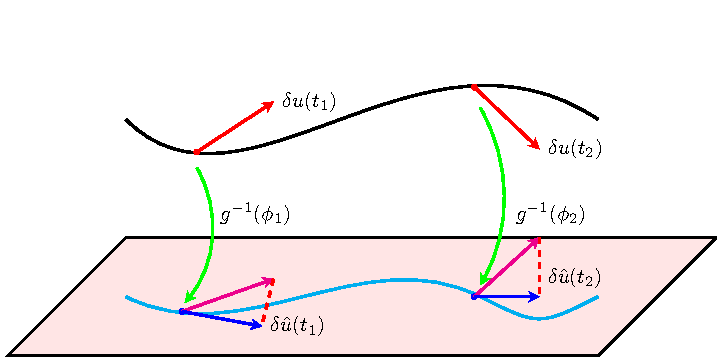
\includegraphics[width=0.9\linewidth]{jacobian_full_slice}
  \caption[Jacobian in the slice]{
    The relation between deformations in
    the full {\statesp} and in the \slice.
    The pink plane is the slice. The black curve is a trajectory in the {\statesp}.
    The cyan curve is the corresponding trajectory in the {\slice}.
    Infinitesimal deformation $\delta \ssp(t_1)$ at time $t_1$
    is transported to $\delta \ssp(t_2)$ at time $t_2$.
    $\delta \sspRed(t_1)$ and $\delta \sspRed(t_2)$ are the in-slice
    correspondents.
  }
  \label{fig:jacobian_full_slice}
\end{figure}

First, we investigate how infinitesimal deformation is
transformed into the slice from the full \statesp.
We start from the \slice\ condition \refeq{eq:slice}.
Infinitesimal deformation $\delta \sspRed$ at $\sspRed$
should be confined to the \slice\ too, so we have a constraint
\begin{equation}
  \braket{\delta \sspRed}{\sliceTan{}}=0
  \,.
  \label{eq:constraint_dx}
\end{equation}
Here, the subscript of $\sliceTan{}$ is omitted because we assume
that there
is only one group parameter.
Taking the derivative of \refeq{eq:slice3} we get
$ \delta \ssp = \delta \LieEl(\gSpace) \sspRed + \LieEl(\gSpace)
\delta \sspRed $ which is equivalent to
\[
  \delta \sspRed=-\Lg \sspRed\delta \gSpace + \LieEl(\gSpace)^{-1}\delta\ssp
  \,.
\]
Substituting it into \refeq{eq:constraint_dx},
we get
$\braket{-\mathbf{T}\sspRed\delta \gSpace + \LieEl(\gSpace)^{-1}
\delta\ssp}{t'}=0$
which is
\begin{equation}
  \label{eq:delta_theta}
  \delta \gSpace=
  \frac{\braket{\sliceTan{}}{\LieEl(\gSpace)^{-1}\delta\ssp}}
  {\braket{\groupTan(\sspRed)}{\sliceTan{}}}
\,.
\end{equation}
Now  $\delta \sspRed$, the infinitesimal deformation in the \slice, can be
expressed by the deformation in the full {\statesp} $\delta\ssp$:
\begin{equation*}
  \ket{\delta \sspRed}
  =
  -\frac{\braket{\sliceTan{}}{\LieEl(\gSpace)^{-1}\delta\ssp}}
  {\braket{\groupTan(\sspRed)}{\sliceTan{}}}
  \ket{\groupTan(\sspRed)}
  + \LieEl(\gSpace)^{-1} \ket{\delta \ssp}
  \,,
\end{equation*}
that is,
\beq
\label{eq:variation_full_slice}
\ket{\delta \sspRed} =
\left(\matId-\frac{\ket{\groupTan(\sspRed)}\bra{\sliceTan{}}}
  {\braket{\groupTan(\sspRed)}{\sliceTan{}}} \right)
\LieEl(\gSpace)^{-1}\ket{\delta \ssp}
:=
h(\sspRed)\LieEl(\gSpace)^{-1}\ket{\delta \ssp}
\eeq
The physical interpretation of \refeq{eq:variation_full_slice} is manifest.
Infinitesimal deformation $\delta \ssp$ at $\ssp$ in the full {\statesp} is
first transformed to point $\sspRed$ by $\LieEl(\gSpace)^{-1}$ and then
projected into the {\slice} by $h(\sspRed)$ illustrated in
\reffig{fig:jacobian_full_slice}.
The matrix
\beq
\pMat(\sspRed)=
    \matId-\frac{\ket{\groupTan(\sspRed)}\bra{\sliceTan{}}}
    {\braket{\groupTan(\sspRed)}{\sliceTan{}}}
%\,.
\ee{projFullToSlice}
projects infinitesimal deformation in the full {\statesp} into the {\slice}.
It is singular and has the following properties.
\begin{itemize}
\item $h(\sspRed)\ket{\groupTan(\sspRed)}=0$ :
  any infinitesimal deformation along the group tangent direction
  at $\sspRed$ in the full {\statesp} will disappear after projection.

\item $\bra{\sliceTan{}}h(\sspRed)=0$ : any vector projected into the {\slice} will be
  perpendicular to the group tangent of the template point as expected. This
  property and the above one both prove that matrix $h(\sspRed)$ is not full-rank.

\item In-slice velocity \refeq{EqMotMFrame} turns out to be
  \[
    \velRed(\sspRed)= \vel(\sspRed)
    -\frac{\braket{\vel(\sspRed)}{\sliceTan{}}}{\braket{\groupTan(\sspRed)}{\sliceTan{}}}
    \groupTan(\sspRed)=h(\sspRed)\vel(\sspRed)
    \,.
  \]
  The velocity field is transformed by matrix $h(\sspRed)$.
\end{itemize}

Since projection matrix \refeq{projFullToSlice} is singular,
the projection
reduces the dimension of the system by one.
However, \refeq{projFullToSlice} is still expressed in
the full {\statesp}.
In practice,
we desire to work in a lower\dmn\ system after quotienting out
the continuous symmetry.
Now let's decrease the dimension of all matrices and
vectors in the {\slice} by one explicitly.
Denote
\[
  \pMat(\sspRed)=
  \begin{bmatrix}
    h_{1} \\
    h_{2} \\
    \vdots \\
    h_{n}
  \end{bmatrix}
  \,.
\]
Each $h_{i}$ is a row vector and $n$ is the dimension of the full {\statesp}.
From the second property of $h(\sspRed)$ we know that $h_{i}$ are linear
dependent: $\sliceTan{1}h_{1}+\sliceTan{2}h_{2}+\cdots +\sliceTan{n}h_{n}=0$.
Here $\sliceTan{i}$ are
components of vector $\sliceTan{}$.
Assume $t'_{\xi}\neq 0$, then
\[
h_{\xi}=\sum_{i=1,i\neq \xi}^{n}-\frac{\sliceTan{i}}{\sliceTan{\xi}}h_{i}
\]
so $h_{\xi}$ can be eliminated from $\pMat(\sspRed)$:
\[
  \pMat(\sspRed)=
  \underbrace{
    \begin{bmatrix}
      1 & & & & \\
      & 1 & & & \\
      & & \ddots & & \\
      -\frac{\sliceTan{1}}{\sliceTan{\xi}} &
      -\frac{\sliceTan{2}}{\sliceTan{\xi}} & & \cdots &
      -\frac{\sliceTan{n}}{\sliceTan{\xi}} \\
      & & & \ddots  & \\
      & & & & 1 \\
    \end{bmatrix}
  }_{n\times (n-1)}
  \underbrace{
    \begin{bmatrix}
      h_{1} \\
      \vdots \\
      h_{\xi-1} \\
      h_{\xi+1} \\
      \vdots \\
      h_{n} \\
    \end{bmatrix}
  }_{(n-1)\times n}
  := P'\pMatM(\sspRed)
  \,.
\]
The above expression is the {rank factorization}
of $h(\sspRed)$ with $\pMatM(\sspRed)$ a full-rank matrix.
The superscript of the minus sign indicates that
the matrix (vector) is $(n-1)$\dmn.
Similarly, from the {\slice} condition $\braket{\sliceTan{}}{\sspRed}=0$,
we can reduce the dimension of a
point on the {\slice} by one
\[
  \sspRed=P'\sspRedM
\]
and also reduce the dimension of an infinitesimal deformation by one
\[
  \delta \sspRed=P'\delta \sspRedM
  \,.
\]
Here, $\sspRedM$ and
$\delta \sspRedM$ are both $(n-1)$\dmn\ vectors.
\[
  \sspRedM=\transp{[\sspRed_1, \cdots, \sspRed_{\xi-1}, \sspRed_{\xi+1}, \cdots, \sspRed_{n}]}
  \,, \quad
  \delta \sspRedM= \transp{[\delta \sspRed_1, \cdots, \delta \sspRed_{\xi-1},
    \delta \sspRed_{\xi+1}, \cdots, \delta \sspRed_{n}]}
  \,.
\]
Now relation \refeq{eq:variation_full_slice} can be rewritten as:
\begin{equation}
  \label{eq:projectionReduced}
  \ket{\delta \sspRedM} = \pMatM(\sspRed)\LieEl(\gSpace)^{-1}\ket{\delta \ssp}
\end{equation}
Note that the left side of the above equation
is an $(n-1)$\dmn\ vector while the right side $\ket{\delta \ssp}$
is an $n$\dmn\ vector and the $[(n-1)\times n]$ matrix $\pMatM(\sspRed)$
is the ``projection'' operator.

%%%%%%%%%%%%%%%%%%%%%%%%%%%%%%%%%%%%%%%%%%%%%%%%%%%%%%%%%%%%%%%%%%%%%%%%
\subsection{In-slice \JacobianM }
\label{sect:sliceJac}

Now let's turn to the transformation of the \JacobianM.
In \reffig{fig:jacobian_full_slice},
there is a trajectory from $\ssp(\zeit_1)$ to $\ssp(\zeit_2)$ in the full {\statesp}.
The corresponding transformed in-\slice\ trajectory is from $\sspRed(\zeit_1)$
to $\sspRed(\zeit_2)$.
Infinitesimal deformations in the full {\statesp} and in the
{\slice}  will be evolved by the
\JacobianM\ in the full {\statesp} and in the {\slice} respectively.
\begin{eqnarray}
  \jMps\delta \ssp(t_1) & = & \delta \ssp(t_2)
                              \label{eq:sliceJ}  \\
  \hat{\jMps}\delta \sspRedM(t_1) & = &\delta \sspRedM(t_2)
                                           \label{eq:sliceJ2}
                                           \,.
\end{eqnarray}
Here, $\jMps = J^{t_2 -t_1}(\ssp(t_1), \zeit_1)$ and
$\hat{\jMps} = J^{t_2 -t_1}(\sspRedM(t_1), \zeit_1)$.
For notation simplicity, we omit all parameters of \JacobianM\
if no confusion occurs.
Substituting \refeq{eq:projectionReduced} into \refeq{eq:sliceJ2},
we get
\[
  \hat{\jMps}  \pMatM(\sspRed(t_1)) \LieEl(\gSpace_1)^{-1} \delta\ssp(t_1)=
  \pMatM(\sspRed(t_2)) \LieEl(\gSpace_2)^{-1}\delta\ssp(t_2)
  =
  \pMatM(\sspRed(t_2)) \LieEl(\gSpace_2)^{-1}\jMps\delta\ssp(t_1)
  \,.
\]
The last step above has used relation \refeq{eq:sliceJ}.
This results in
\begin{equation}
  \label{eq:relation_jacobian1}
  \hat{\jMps}\pMatM
  (\sspRed(\zeit_1))\LieEl(\gSpace_1)^{-1}=
  \pMatM(\sspRed(\zeit_2))\LieEl(\gSpace_2)^{-1}\jMps
  \,.
\end{equation}
$\hat{\jMps}$ is an $[(n-1)\times (n-1)]$ matrix as we can easily see.
The geometrical meaning of relation \refeq{eq:relation_jacobian1} is obvious
in \reffig{fig:jacobian_full_slice}. On the left side, the
infinitesimal deformation $\delta \ssp(\zeit_1)$ at $\ssp(\zeit_1)$ is
transported to the slice first,
and then projected into the \slice, after which it is
evolved by $\hat{\jMps}$ to in-slice point
$\sspRed(\zeit_2)$. On the right side, the
infinitesimal deformation $\delta \ssp(\zeit_1)$ at $\ssp(\zeit_1)$ is evolved
first to $\ssp(\zeit_2)$
by $\jMps$, then transported to the slice, and finally projected
into the \slice.

By \refeq{eq:relation_jacobian1},
the relation between {\cLvs} in the full {\statesp} and in the {\slice}
can be obtained for
physically interesting invariant subsets: \eqva, \reqva, \po s, and
\rpo s.

\paragraph{In-slice stability matrix of an \eqv}
For an \eqv\ $\ssp(\zeit_1) = \ssp(\zeit_2) := \ssp_q$, we have
$\sspRed(\zeit_1)=\sspRed(\zeit_2) :=\sspRed_q$ and
$\gSpace_{1}=\gSpace_{2} := \gSpace_q$.
Formula \refeq{eq:relation_jacobian1} becomes
\begin{equation}
  \hat{\jMps}\pMatM
  (\sspRed_q)\LieEl(\gSpace_q)^{-1}=
  \pMatM(\sspRed_q)\LieEl(\gSpace_q)^{-1}\jMps
  \,.
  \label{eq:Jeqv0}
\end{equation}
Moreover, by \refeq{eq:tangentDynamics} we have $J=e^{(t_2-t_1)A}$
for \eqva, so \refeq{eq:Jeqv0} becomes
\begin{equation}
  \hat{A} \pMatM
  (\sspRed_q)\LieEl(\gSpace_q)^{-1}=
  \pMatM(\sspRed_q)\LieEl(\gSpace_q)^{-1}A
  \,,
  \label{eq:Jeqv1}
\end{equation}
where $\hat{A}$ is the in-slice stability matrix.
\refeq{eq:Jeqv1} relates stability matrix in the \slice\ and that in the
full \statesp\ by a similarity transformation.
So
\begin{equation}
  \label{eq:Jeqv}
  \hat{\ExpaEig}_{j} = \ExpaEig_{j} \,, \quad
  \jEigvecRed[j] = \pMatM(\sspRed_q)\LieEl(\gSpace_q)^{-1} \jEigvec[j]
  \,.
\end{equation}
Here, $\hat{\ExpaEig}_{j}$ and $\ExpaEig_{j}$ are the
stability exponents in the \slice\ and in the full \statesp\ respectively.
$\hat{\jEigvec}$ and $\jEigvec$ are the corresponding eigenvectors.

\paragraph{In-slice stability matrix of a \reqv}
For an \reqv\ $\LieEl(c(\zeit_2-\zeit_1)) \ssp(\zeit_2) =  \ssp(\zeit_1)$,
we also have $\sspRed(\zeit_1)=\sspRed(\zeit_2) :=\sspRed_q$ and
$\gSpace_{1} = \gSpace_{2} - c (\zeit_2 - \zeit_1)$. Formula
\refeq{eq:relation_jacobian1} reduces to
\begin{equation}
  \hat{\jMps} \left( \pMatM(\sspRed_q)\LieEl(\gSpace_1)^{-1} \right) =
  \left( \pMatM(\sspRed_q)\LieEl(\gSpace_1)^{-1} \right)
  \LieEl(c(t_2-t_1))^{-1}\jMps
  \,.
  \label{eq:Jreqv0}
\end{equation}
If let $\zeit_2 - \zeit_1 = \delta \zeit$ be an infinitesimal time
lapse. Then
\[
  \jMps = \matId + A \delta \zeit \,\quad
  \text{and} \quad
  \LieEl(c(\zeit_2 - \zeit_1)) = \matId + c\Lg \delta\zeit
\]
are
first-order accurate. Thus \refeq{eq:Jreqv0} gives
\begin{equation}
  \label{eq:Jreqv1}
  \hat{A} \left( \pMatM(\sspRed_q)\LieEl(\gSpace_1)^{-1} \right) =
  \left( \pMatM(\sspRed_q)\LieEl(\gSpace_1)^{-1} \right)
  (-c\Lg + A)
  \,.
\end{equation}
Actually, $-c\Lg + A$ is the \emph{effective} stability matrix of
a \reqv\ in the full \statesp, so \refeq{eq:Jreqv1}
relates the stability matrix in the \slice\ with the effective stability matrix
in the full \statesp\ by a similarity transformation. Therefore,
their spectra and eigenvectors have the same relation as in
\refeq{eq:Jeqv}.

\paragraph{In-slice \JacobianM\ of a \po}
For a \po\ $\ssp(0)=\ssp(\period{p})$, if we
set $\zeit_2 = \zeit_1 + \period{p}$ we have
$\sspRed(\zeit_1)=\sspRed(\zeit_2) :=\sspRed_p$ and
$\gSpace_{1}=\gSpace_{2} := \gSpace_p$. So, the Floquet matrix
has relation
$\hat{\jMps}_p\pMatM
(\sspRed_p)\LieEl(\gSpace_p)^{-1}=
\pMatM(\sspRed_p)\LieEl(\gSpace_p)^{-1}\jMps_p$.
Therefore, the \Fv s and Floquet multipliers
in the slice and those in the full \statesp\
have the
same relation as in \refeq{eq:Jeqv}.

\paragraph{In-slice \JacobianM\ of a \rpo}
For a \rpo\
$\ssp(0)=\LieEl(\gSpace_p)\ssp(\period{p})$, if we also
set $\zeit_2 = \zeit_1 + \period{p}$ then we have
$\sspRed(\zeit_1)=\sspRed(\zeit_2):=\sspRed_p$ and
$\gSpace_1 = \gSpace_p + \gSpace_2$.
Relation \eqref{eq:relation_jacobian1} becomes
\begin{equation}
  \label{eq:Jrposlice}
  \hat{\jMps} \pMatM
  (\sspRed_p)\LieEl(\gSpace_{1})^{-1}
  = \pMatM (\sspRed_p)\LieEl(\gSpace_{1})^{-1} \jMps_p
  \,.
\end{equation}
Here $\jMps_p = \LieEl(\gSpace_p) J$ is the Floquet matrix in the full
\statesp\ for a \rpo. So the same as \po s, we have relation \refeq{eq:Jeqv}.

In summary, relation \refeq{eq:Jeqv} holds for \eqva, \reqva, \po s, and
\rpo s. The stability spectrum (Floquet spectrum) in the slice is the
same as that in the full \statesp. Eigenvectors (\Fv s)
in the full \statesp\
are first transported to the slice and then projected into the slice.
This is the exact reason that using a slice to reduce continuous symmetries
not only keeps the dynamical properties unchanged but also
simplifies the analysis.

%%%%%%%%%%%%%%%%%%%%%%%%%%%%%%%%%%%%%%%%%%%%%%%%%%%%%%%%%%%%%%%%%%%%%%%%
\subsection{An example: the \twomode\ system}

In this subsection, we use the \twomode\ system as an example to
illustrate the techniques described in the previous two subsections.
We follow Chaosbook\rf{DasBuch}
for the setup of the \twomode\ system
\bea
\dot{x}_1 &=& (\mu_1    - r^2)\,x_1 + c_1\,(x_1 x_2 + y_1 y_2)
    \,,\qquad       r^2 = x_1^2 + y_1^2
\continue
\dot{y}_1 &=& (\mu_1    - r^2)\,y_1 + c_1\,(x_1 y_2 - x_2 y_1)
\continue
\dot{x}_2 &=& x_2 +  y_2 + x_1^2 - y_1^2  + a_2 x_2 r^2
\continue
\dot{y}_2 &=& -  x_2 + y_2 + 2\,x_1 y_1  + a_2 y_2 r^2
\,.
\label{angSO2set1real}
\eea
and the choice of parameters:
\[
  \mu_1 = -2.8\,,\quad
  a_2 = -2.66\,,\quad
  c_1 = -7.75\,.
\]
Full \statesp\ points are represented as
$\ssp = \transp{(x_1, y_1, x_2, y_2)}$.
The \twomode\ system \refeq{angSO2set1real} has an \SOn{2} symmetry
\[
  \LieEl(\gSpace) \,=\,  \left(\barr{ccccc}
    \cos \gSpace  &\sin \gSpace  & 0 & 0  \\
    -\sin \gSpace  &~\cos \gSpace  & 0 & 0  \\
    0 & 0 &  \cos 2\gSpace &\sin 2\gSpace    \\
    0 & 0 &  -\sin 2\gSpace &~\cos 2\gSpace
    \earr\right)
  \,
\]
with the corresponding Lie group generator
\beq
 \Lg \,=\,   \left(\barr{ccccc}
    0  & 1 & 0  &  0   \\
    -1  &  0 & 0  &  0  \\
    0  &  0 & 0  & 2   \\
    0  &  0 & -2  &  0
    \earr\right)
  \,.
\ee{2modefLieGen}
In order to reduce this continuous symmetry,
$\slicep=\transp{(1,0,0,0)}$ is chosen as the template point the
same as that in
Chaosbook\rf{DasBuch}, and thus the resulting \slice\ condition is
\[
  \braket{\sspRed}{\sliceTan{}} = 0
  \;\text{and}\;
  \hat{x}_1 > 0
  \quad \text{with} \quad
  \sliceTan{} = \transp{(0, -1, 0, 0)}
  \,.
\]
The in-slice state is denoted as
$\sspRed = \transp{(\hat{x}_1, 0, \hat{x}_2, \hat{y}_2)}$.
Symmetry reduction is equivalent to rotating every state into
the positive real axis in the $(x_1, y_1)$ plane.

\begin{figure}[h]
  \centering
  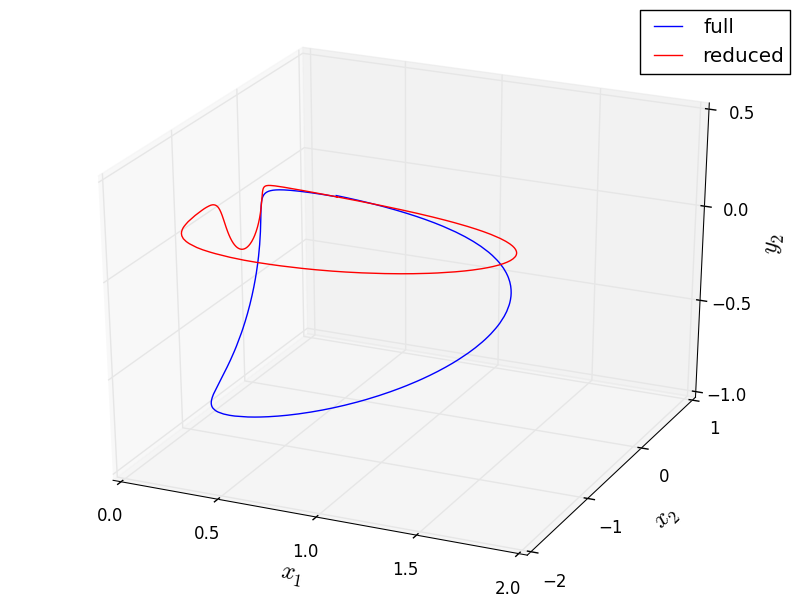
\includegraphics[width=0.8\textwidth]{twomodes_configuration}
  \caption[A \rpo\ in the \twomode\ system.]
  {
    The configuration of $\cycle{1}$ in the full \statesp\ projected
    into subspace $[x_{1},x_{2},y_{2}]$ (the blue curve) and in the slice (
    the red curve).
  }
  \label{fig:twomodes_configuration}
\end{figure}
In this subsection, we focus on one \rpo\ in the \twomode\ system
whose initial condition is
\begin{equation}
  \label{eq:2modeInit1}
  \cycle{1}: \quad (0.4525719,\quad 0.0,\quad 0.0509257,\quad 0.0335428)
  \,.
\end{equation}
The orbit has period $3.6415$.
\refFig{fig:twomodes_configuration} depicts \rpo\
$\cycle{1}$ in the full \statesp\ and in the slice.
The Floquet multipliers associated with this orbit are
\begin{equation}
  \label{eq:2modeMulti1}
  \ExpaEig_{j} : \quad (-1.481177, \quad
  -1.066888\cdot 10^{-09},\quad  0.999414,\quad  0.999913)
  \,.
\end{equation}
It has a weak expanding direction, a strong
contracting direction, and two marginal directions.

\begin{figure}[h]
  \centering
  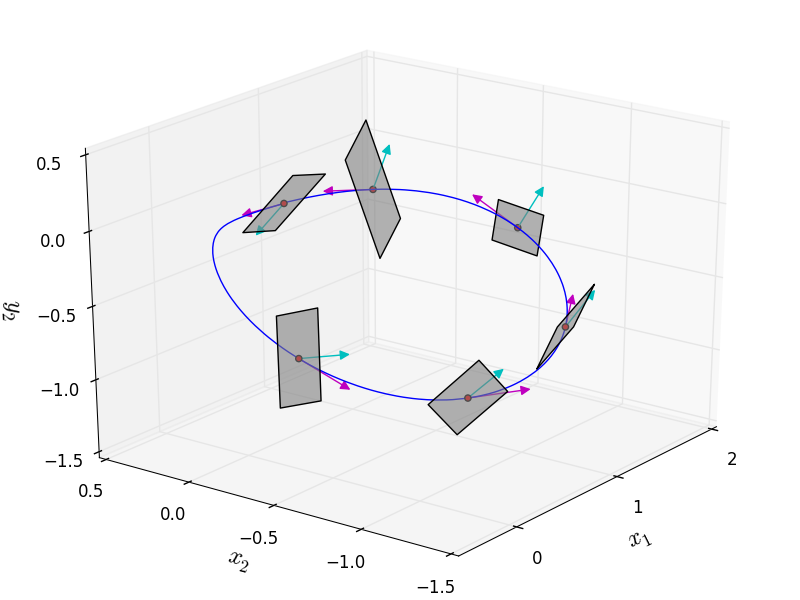
\includegraphics[width=0.8\textwidth]{twomodes_full}
  \caption[Marginal \Fv s in the \twomode\ system.]{
    The gray planes are spanned by the two marginal \Fv s.
    of \rpo\ $\cycle{1}$.
    The pink, green arrows are the velocity vectors and the group
    tangents on this orbit respectively.
    The blue curve is \rpo\ $\cycle{1}$ projected into the
    subspace $[x_{1},x_{2},y_{2}]$.
  }
  \label{fig:twomodes_full}
\end{figure}
The velocity field $\vel(\ssp)$ and the group tangent $\groupTan(\ssp)$
are \Fv s of this system and give rise to the two
marginal multipliers in \refeq{eq:2modeMulti1}, but the corresponding
two \Fv s are degenerate which cannot be told apart when we solving the
eigenequation of the \JacobianM. However, we can check whether $\vel(\ssp)$
and $\groupTan(\ssp)$ are contained in the subspace spanned by
these two \Fv s. This is the idea of \reffig{fig:twomodes_full},
in which we show the planes spanned by the two marginal \Fv s, the velocity field,
and the group tangent, along this orbit.
As we can see, $\vel(\ssp)$ and $\groupTan(\ssp)$ do lie in the planes.
Therefore, the calculation of Floquet spectrum and \Fv s
of $\cycle{1}$ is accurate at least for illustration purpose.

\begin{figure}[h]
  \centering
  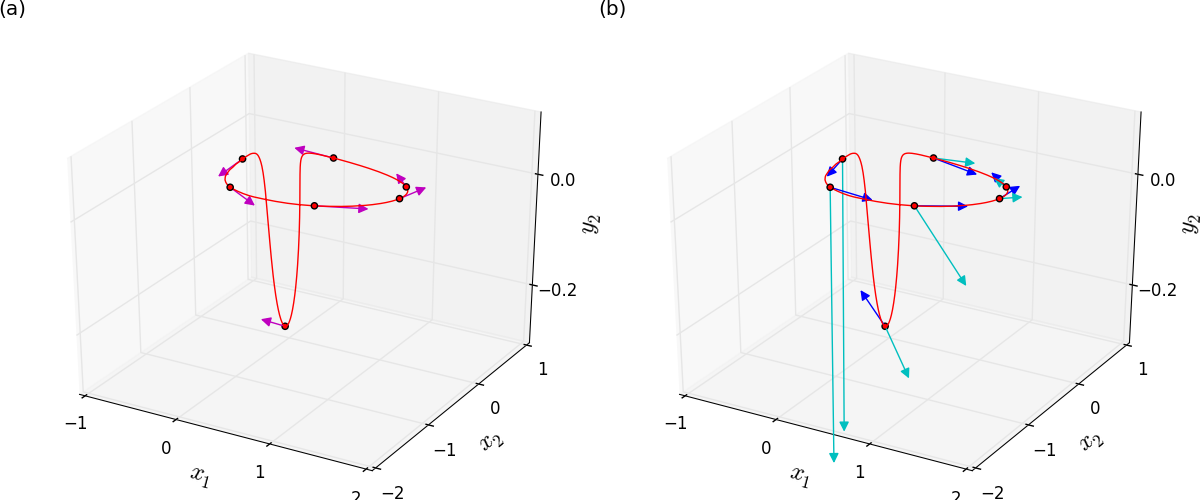
\includegraphics[width=1\textwidth]{twomodes_reduced}
  \caption[\Fv s in the slice in the \twomode\ system]{
    In-slice \Fv s for \rpo\ $\cycle{1}$.
    The red closed curve is $\cycle{1}$.
    (a) The marginal \Fv\ (pink).
    (b) The expanding (blue) and contracting (green) \Fv s in the slice.
  }
  \label{fig:twomodes_reduced}
\end{figure}

Now the task is to transform these \Fv s into the slice.
By the Lie group generator \refeq{2modefLieGen}, we get the
group tangent of an in-slice point
$\sspRed = \transp{(\hat{x}_1, 0, \hat{x}_2, \hat{y}_2)}$:
\[
  t(\sspRed)=(0,-\hat{x}_{1},2\hat{y}_{2},-2\hat{x}_{2})
  \,.
\]
Then by \refeq{projFullToSlice} we have
\[
  \pMat(\sspRed)=
  \begin{pmatrix}
    1 & 0 & 0 & 0 \\
    0 & 0 & 0 & 0 \\
    0 & 2\hat{y}_{1}/\hat{x}_{1} & 1 & 0 \\
    0 & -2\hat{x}_{2}/\hat{x}_{1} & 0 & 1 \\
  \end{pmatrix}
  \,.
\]
We choose to eliminate the second coordinate $\hat{y}_{1}$, then
\[
  \pMatM(\sspRed)=
  \begin{pmatrix}
    1 & 0 & 0 & 0 \\
    0 & 2\hat{y}_{1}/\hat{x}_{1} & 1 & 0 \\
    0 & -2\hat{x}_{2}/\hat{x}_{1} & 0 & 1 \\
  \end{pmatrix}
\,.
\]
Matrix $\pMatM(\sspRed)$ transforms \Fv s in the full \statesp\ into the
slice which are shown in \reffig{fig:twomodes_reduced}.
The group tangent $\groupTan(\sspRed)$, as one marginal vector,
disappears and the planes in \reffig{fig:twomodes_full}
collapse to the velocity
field along the orbit shown in \reffig{fig:twomodes_reduced}(a).
The other two projected \Fv s are shown in
\reffig{fig:twomodes_reduced}(b).

\begin{figure}[h]
  \centering
  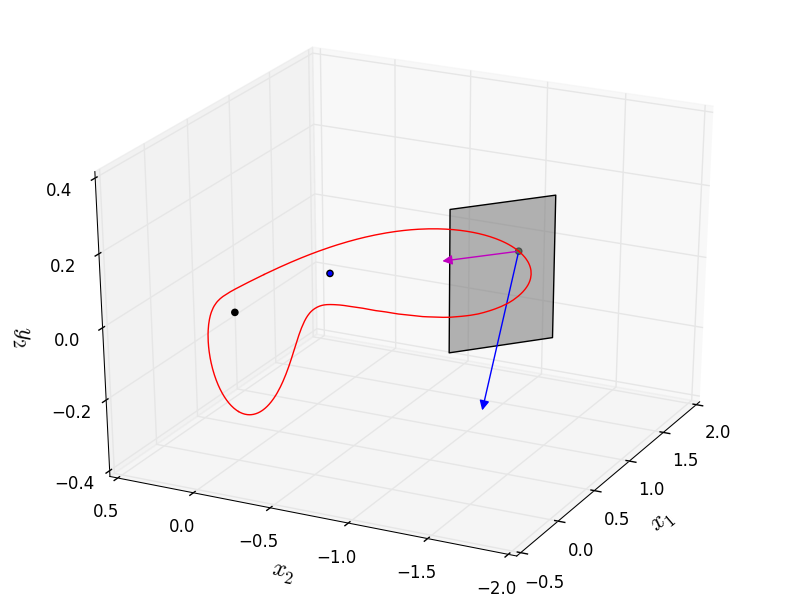
\includegraphics[width=0.8\textwidth]{twomodes_poincare}
  \caption[\Fv s on the {\PoincSec} in the \twomode\ system]{
    A vertical {\PoincSec} is constructed from the origin
    (black point) and a relative equilibrium
    (blue point) in
    the slice.
    The \PoincSec\ intersects $\cycle{1}$ (the red closed curve)
    at the green point.
    In-slice \Fv s are projected into the
    {\PoincSec}. The red/blue vector is the expanding/contracting
    \Fv. The marginal vector along the orbit disappears on the {\PoincSec}.
  }
  \label{fig:twomodes_poincare}
\end{figure}

In a similar way\rf{DasBuch}, \Fv s on
the slice could be
projected onto a {\PoincSec}. The projection matrix is
\[
  h_{\mathcal{P}}(\sspRed) = \matId -
  \frac{\ket{\hat{\vel}}\bra{\partial U}}{\braket{\hat{\vel}}{\partial U}}
  \,,
\]
where $U(x) = 0$ defines the {\PoincSec} with $\partial U$ its normal direction.
$\hat{\vel}$ is the in-slice velocity.
A \PoincSec\ can be fixed by choosing three points on it, or equivalently,
by three conditions. Here, we choose a ``vertical'' \PoincSec, namely, we demand
that the
$\hat{y}_2$ component of its normal direction vanishes. Next, this \PoincSec\
goes through the origin $(0,0,0)$ and a \reqv\
\[
  (\hat{x}_{e1}, \hat{x}_{e2},
  \hat{y}_{e2})=(0.439965,\quad -0.386267, \quad 0.070204)
  \,,
\]
shown in \reffig{fig:twomodes_poincare}.
In this case, $\partial U=(\hat{x}_{e2},- \hat{x}_{e1}, 0)$ and we get
\[
  h_{\mathcal{P}}(\sspRed)
  =\frac{1}{\hat{v}_{1}\hat{x}_{e2}-\hat{v}_{2}\hat{x}_{e1}}
  \begin{pmatrix}
    -\hat{v}_{2}\hat{x}_{e1} & \hat{v}_{1}\hat{x}_{e1} & 0 \\
    -\hat{v}_{2}\hat{x}_{e2} & \hat{v}_{1}\hat{x}_{e2} & 0 \\
    -\hat{v}_{3}\hat{x}_{e1} & \hat{v}_{3}\hat{x}_{e1} &
    \hat{v}_{1}\hat{x}_{e2}-\hat{v}_{2}\hat{x}_{e1}\\
  \end{pmatrix}
  \,.
\]
\refFig{fig:twomodes_poincare} shows the projected
expanding and contracting \Fv s
on the {\PoincSec}. The marginal vector (velocity field)
disappears.

\begin{figure}[h]
  \centering
  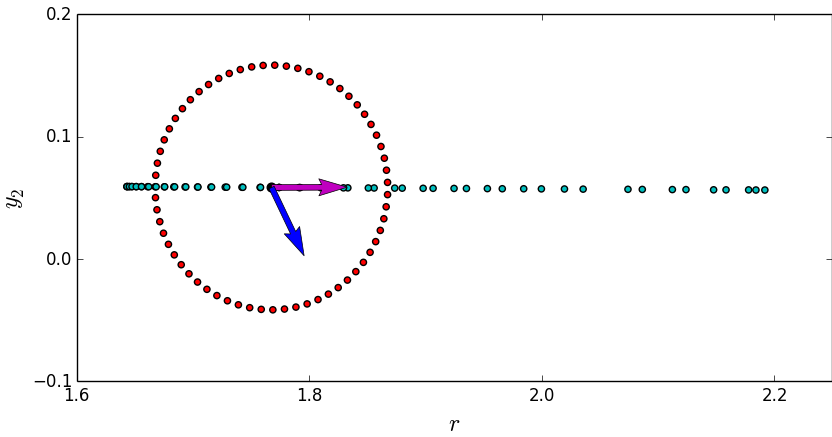
\includegraphics[width=0.8\textwidth]{twomodes_poincare_return}
  \caption[First returning points on the {\PoincSec} in
  the \twomode\ system]{
    A set of circularly (radis=0.1) distributed points (red)
    around the intersection
    point evolves for one period.
    Their first returning points (green) are recorded.
    The pink and blue arrows are the expanding
    and contracting
    \Fv s projected onto the {\PoincSec} respectively.
    Here $r=(\hat{x}_{1}^2+\hat{x}_{2}^2)^{1/2}$.
  }
  \label{fig:twomodes_poincare_return}
\end{figure}

Last, \reffig{fig:twomodes_poincare_return} shows the
{\PoincSec} and the
two projected \Fv s. A set of
circularly distributed points around
the intersection point  evolves for one period
and their first returning points are
recorded.
The contracting direction is close to the vertical direction,
and \refeq{eq:2modeMulti1} says that the contracting rate is large
in this direction. Therefore,
the returning points are squashed heavily in the
vertical direction; however, the magnitude of expanding multiplier is
about 1.5, so the elongation in the horizontal direction is relatively
small.

In summary,
we have reduced the \SOn{2} symmetry of the \twomode\ system
and discussed the \Fv s of a specific \rpo\ in the full state space and in the
slice. The marginal direction along the group orbit tangent is eliminated by the
slice. Furthermore, we have constructed a \PoincSec\ of codimension two with
respect to the original system. In this \PoincSec, the \rpo\ $\cycle{1}$
is reduced to a fixed point with
one expanding and one contracting \Fv, and the dynamics is
greatly simplified. This simple example illustrates why symmetry reduction
is an indispensable tool when studying dynamical systems with
continuous symmetries.


%% siminos/xiong/thesis/chapters/symFactor.tex
% $Author: predrag $ $Date: 2017-03-09 17:25:05 -0500 (Thu, 09 Mar 2017) $

% Xiong 2017-03-08 omitted from the thesis

\section{Discrete factorization of the dynamic zeta function}
\label{sect:fact}

When a dynamical system has a discrete symmetry, the cycle averaging
formula \refeq{eq:sd} and \refeq{eq:zeta} can be simplified substantially,
and the expansion needs
much fewer orbits to achieve the desired accuracy.
In this section, we discuss how the \dzeta\ can be factorized by a
product of contributions from each irreps of this discrete symmetry.

\subsection{Factorization of $C_3$ and $D_3$}

\begin{figure}[h]
  \centering
  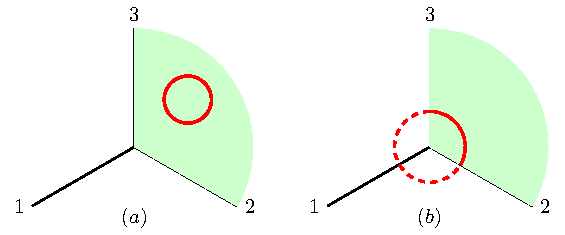
\includegraphics[width=0.9\textwidth]{C3orbits}
  \caption[Orbits in a system with $C_3$ symmetry.]{
    The two different kinds of \po s in a system with
    $C_3$ symmetry.
    The green region is the chosen fundamental domain.
    The red cycles are \po s.
  }
  \label{fig:C3orbits}
\end{figure}

$C_3$ has two subgroups $\{e\}$ and $\{e, C^{1/3}, C^{2/3}\}$, so there are
two types of \po s as shown in \reffig{fig:C3orbits}. A type-(a) orbit
has symmetry
$\{e\}$, \ie, no symmetry, and it has two replicas by rotation $C^1/3$  and $C^{2/3}$
respectively, which are not shown in this figure. So the contribution from
a type-(a) orbit to the \dzeta\ \refeq{eq:zeta} is $(1-t_p)^3$.
The cubic order refers to the a fact that there are three sibling orbits together.
Also, since the entire orbit is in the fundamental domain, we have
\[
  1/\zeta_a = (1 - t_{\hat{p}})^3
  \,.
\]
The hat on $p$ means that $t_{\hat{p}}$ is evaluated only on the part of the orbit that
is in the fundamental domain.
A type-(b) orbit is invariant under $e$, $C^{1/3}$ and $C^{2/3}$.
This orbit has no siblings and only one third
of this orbit is in the fundamental domain. The other two thirds are replicas
by rotation $C^1/3$  and $C^{2/3}$ of the part in the fundamental domain. So, its
contribution to \dzeta\ is
\[
  1/\zeta_b = 1 - t_p = 1 - t_{\hat{p}}^3
  \,.
\]
Here, relation $t_p= t_{\hat{p}}^3$ is easily obtained by its definition in
\refeq{eq:zeta}.
On the other hand, by \refexam{exam:C3regularRep},
we know that the regular representations of $e$,
$C^{1/3}$, and $C^{2/3}$ are respectively
\[
  D^{reg}(e) = %&=&
  \begin{bmatrix}
    1 & & \\
    & 1 & \\
    & & 1 \\
  \end{bmatrix} \,,  \quad
  % \continue
  D^{reg}(C^{1/3}) = %&=&
  \begin{bmatrix}
    ~ & 1 & ~\\
    ~ & ~ & 1\\
    1 & ~ & ~ \\
  \end{bmatrix}\,,  \quad
  D^{reg}(C^{2/3}) =
  \begin{bmatrix}
    ~ & ~ & 1\\
    1 & ~ & ~\\
    ~ & 1 & ~ \\
  \end{bmatrix}
  \,.
\]
You can easily verify that
\[
 (1 - t_{\hat{p}})^3 = \det(1 - D^{reg}(e)t_{\hat{p}}) \,, \quad
 1 - t_{\hat{p}}^3 = \det(1 - D^{reg}(C^{1/3})t_{\hat{p}}) =
 \det(1 - D^{reg}(C^{2/3})t_{\hat{p}})\,.
\]
Therefore, you see that the contribution from \po s to the
\dzeta\ in a system with $C_3$
symmetry are related to the regular representation of $C_3$.

\begin{figure}[h]
  \centering
  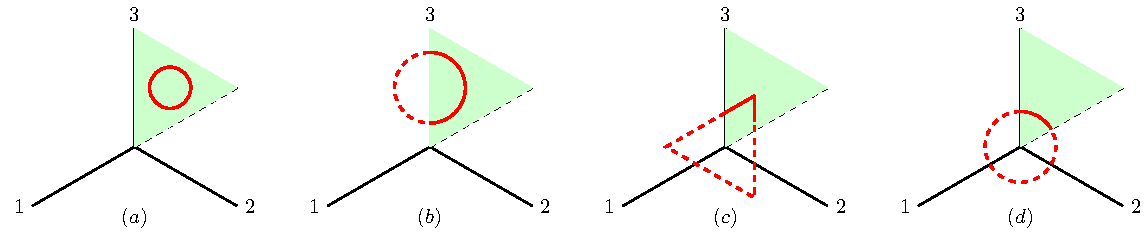
\includegraphics[width=0.9\textwidth]{D3orbits}
  \caption[Orbits in a system with $D_3$ symmetry.]{
    The four different kinds of \po s in a system with
    $D_3$ symmetry.
    The green region is the chosen fundamental domain.
    The red cycles are \po s.
  }
  \label{fig:D3orbits}
\end{figure}

Let us check out another example - a system with $D_3$ symmetry.
$D_3$ has four different kinds of subgroups $\{e\}$, $\{e, \sigma\}$,
$\{e, C^{1/3}, C^{2/3}\}$, and $D_3$ itself. Here $\sigma$ can be
any one of $\sigma_{12}$, $\sigma_{23}$ or $\sigma_{31}$. Accordingly,
there are four types of \po s as shown in \reffig{fig:D3orbits}.
The fundamental domain is one sixth of the full \statesp.
Similar to the analysis of the two orbits in the $C_3$ case, we have
\[
  1/\zeta_a = (1 - t_{\hat{p}})^6
  \,,\quad
  1/\zeta_b = (1 - t_{\hat{p}}^2)^3
  \,,\quad
  1/\zeta_c = (1 - t_{\hat{p}}^3)^2
  \,,\quad
  1/\zeta_d = 1 - t_{\hat{p}}^6
  \,.
\]
\refExam{exam:D3regularRep} gives the regular representation of $D_3$.
You can also verify that
\begin{align*}
   & (1 - t_{\hat{p}})^6 = \det(1 - D^{reg}(e)t_{\hat{p}}) \,, \quad
     (1 - t_{\hat{p}}^2)^3 = \det(1 - D^{reg}(\sigma)t_{\hat{p}}) \\
   & (1 - t_{\hat{p}}^3)^2 = \det(1 - D^{reg}(C^{1/3})t_{\hat{p}})\,,\quad
     1 - t_{\hat{p}}^6 = ?
     \,.
\end{align*}
I leave a question mark above since no analogous expression exists for it.
We will come back to it after proving
the identity \refeq{eq:symfac}.

We can generalize the above observation for a system invariant under
a general discrete group
$\Group=\{e, \LieEl_2, \LieEl_3,\cdots, \LieEl_{|\Group|}\}$.
Let $h$ be an element of $\Group$
with order (period) $m$, \ie, $m$ is the smallest positive integer such
that $h^m = e$. Then we have
\begin{equation}
  \label{eq:symfac}
  (1 - t^m)^{\frac{|G|}{m}} = \det(1 - D^{reg}(h)t)
  \,.
\end{equation}
The proof starts from the matrix identity $\ln\det = \tr\ln$, by which we have
\[
  \ln \det(1 - D^{reg}(h)t) = \tr \ln (1 - D^{reg}(h)t)
  = -\sum_{k=1}^\infty \frac{\tr D^{reg}(h^k)t^k}{k}
  \,.
\]
The last identity above comes from the Taylor expansion
$\ln(1-x) = -\sum_{k=1}^\infty \frac{x^k}{k}$.
As we know, the regular representation of
a group element has nonzero trace if and only if this group element is
$e$. So we have,
\[
  \ln \det(1 - D^{reg}(h)t) =  -\sum_{k=1}^\infty \frac{|G|t^{mk}}{mk}
  =  -\frac{|G|}{m}\sum_{k=1}^\infty \frac{t^{mk}}{k}
  = \frac{|G|}{m} \ln (1 - t^m)
  \,.
\]
Therefore, we obtain \refeq{eq:symfac}. This is why we have the observation
in the $C_3$ and $D_3$ example. However, for the type-(d) orbit in
\reffig{fig:D3orbits}, the symmetry group of this orbit is
$\{e, \sigma_{12}, \sigma_{32}, \sigma_{13}, C^{1/3}, C^{2/3}\}$. The order of
$\sigma$ is 2 while the order of $C^{1/3}$ is 3. The least common multiple is
6. Therefore, the contribution to the \dzeta\ is $(1-t_{\hat{p}}^6)^{1}$ and it
cannot be written as form $\det(1 - D^{reg}(h)t_{\hat{p}})$ with some $h\in G$.

Actually, we can write
\[
  1-t_{\hat{p}}^6 = \det(1 - D^{reg}(C^{1/3})t_{\hat{p}}^2) \,,\quad
  \text{or} \quad
  1-t_{\hat{p}}^6 = \det(1 - D^{reg}(\sigma)t_{\hat{p}}^3)
\]
With $D^{reg}(C^{1/3})$ the $[3\times 3]$ representation of $C^{1/3}$ in group $C_3$
and $ D^{reg}(\sigma)$ the $[2\times 2]$ representation of $\sigma$ in
reflection group $\{e, \sigma\}$. Anyway, for the type-(d) orbit we
have no choice but to give up the regular representation of $D_3$.

\subsection{Factorization of $C_n$ and $D_n$}

for a discrete symmetry group
$G=\{{ e},{ g}_2,\ldots,{ g}_{|G|}\}$. The orthogonality and completeness
of projection operator
can be easily verified by the orthogonality relation among characters of
irreducible representation. Define $ \cal L_\alpha=P_\alpha \cal L$, then
the trace of {\evOper} $\cal L$ can be decomposed into a sum of
$ \sum_\alpha \tr {\cal L}_\alpha$ because of the completeness of projection
operators.
\Xiong{2014-05-03}{Here the decomposition of trace just relies on the
  completeness of projection operators, we haven't used the commuting
  relation between {\evOper} and group transform. Am I right?}
So we only need to investigate the projected trace formula:
\begin{align*}
  \tr {\cal L}_\alpha & = \frac{d_\alpha}{|G|}\sum_{h \LieEl\in\Group} \chi_\alpha (h)
                        {\bf h}^{-1} \int_\pS dx \, {\cal L} ( x,x) \\
                      & =\frac{d_\alpha}{|G|}\sum_{h \LieEl\in\Group} \chi_\alpha (h) {\bf h}^{-1}
                        \sum_{a \LieEl\in\Group}\int_{\tilde{\pS}} d(a\tilde{x}) \,{\cal L} (a\tilde{x},a\tilde{x})
  \\
                      & =\frac{d_\alpha}{|G|}\sum_{h \LieEl\in\Group} \chi_\alpha (h) {\bf h}^{-1}\,\cdot
                        |G|\int_{\tilde{\pS}} d(\tilde{x}) \,{\cal L} (\tilde{x},\tilde{x}) \\
                      & = d_\alpha \sum_{h \LieEl\in\Group} \chi_\alpha (h) \int_{\tilde{\pS}} d\tilde{x} \,
                        {\cal L} ({\bf h}^{-1} \tilde{x},\tilde{x})
\end{align*}
In the above derivation, we have used the invariance of {\evOper}
under group transform. For a \po\ in the fundamental domain
$\tilde{p}$, we follow the standard argument in Chaosbook and get
\[
  \int_{\tilde{\pS}} d\tilde{x} \, {\cal L} ({\bf h}^{-1} \tilde{x},\tilde{x}) =
  \cl{\tilde{p}} \sum_{r=1}^\infty { e^{r \beta \cdot \Obser_{\tilde{p}}}
    \over  | \det \left( {\bf 1}- {\tilde\monodromy}_{\tilde{p}}^{r} \right)
    | } \delta_{n,\cl{\tilde{p}} r}\delta_{h,h_{\tilde{p}}^r}
  \,;
\]
so, the {\Fd} is
\bea
F(z) &=& \prod_\alpha F_\alpha (z)^{d_\alpha}
\continue   %\,\, , \quad \quad
F_\alpha (z) &=&
{\rm exp}  \left( - {
    \sum_{\tilde{p}} \sum_{r=1}^\infty {1 \over r}
    {\chi_\alpha (h_{\tilde{p}}^r)  z^{\cl{\tilde{p}} r}
      e^{r \beta \cdot \Obser_{\tilde{p}}}
      % {\phi_p^r}
      \over  | \det \left( {\bf 1}- {\tilde\monodromy}_{\tilde{p}}^{r} \right) | }
  } \right)
\,\,  ,
\eea
which is discrete factorization for maps. The same method can be applied to
flows with discrete symmetry:
\[
  F_\alpha (z) =
  {\rm exp}  \left( - {
      \sum_{\tilde{p}} \sum_{r=1}^\infty {1 \over r}
      {\chi_\alpha (h_{\tilde{p}}^r) e^{r (\beta \cdot \Obser_{\tilde{p}}-sT_{\tilde{p}})}
        % {\phi_p^r}
        \over  | \det \left( {\bf 1}- {\tilde\monodromy}_{\tilde{p}}^{r} \right) | }
    } \right)
\]

Making an approximation
$| \det \left( {\bf 1}- {\tilde\monodromy}_{\tilde{p}}^{r} \right) | \approx
|\Lambda_{\tilde{p}}|$ where $\Lambda_{\tilde{p}}$ is the product of all
expanding multipliers, we get the factorized zeta function:
\begin{equation}
  F_\alpha (z) =
  {\rm exp}  \left( -
    \sum_{\tilde{p}} \sum_{r=1}^\infty {1 \over r}
    \chi_\alpha (h_{\tilde{p}}^r) t_{\tilde{p}}^{r} \right)
  \label{eq:redzeta}
\end{equation}

Formula \eqref{eq:redzeta} is the ultimate goal of Discrete Factorization,
which basically tells us that,
equipped with character table of the group in question, we can write down
all the factorized zeta function for all classes of this group. On the
other hand, in order to verify our result,
let's calculate the zeta
function in the full \statesp.
\begin{align*}
  F(z) &= \prod_\alpha F_\alpha (z)^{d_\alpha} \\
       &= {\rm exp}  \left( -
         \sum_{\tilde{p}} \sum_{r=1}^\infty {1 \over r}\sum_{\alpha}
         \left(d_{\alpha}\chi_\alpha (h_{\tilde{p}}^r)\right) t_{\tilde{p}}^{r} \right) \\
       &= {\rm exp}  \left( -
         \sum_{\tilde{p}} \sum_{r=1}^\infty {1 \over r}
         |G|\delta_{h_{\tilde{p}}^{r},e}  t_{\tilde{p}}^{r} \right) \\
       &= {\rm exp}  \left( -
         \sum_{\tilde{p}} \sum_{k=1}^\infty {|G| \over mk}
         t_{\tilde{p}}^{mk} \right)
         \,,
\end{align*}
that is
\begin{equation}
  \label{eq:fullzeta}
  F(z)= \left(1-t_{\tilde{p}}^{\frac{|G|}{m}}\right)^{m} \,,
\end{equation}
where $m$ is the smallest positive number such that $h_{\tilde{p}}^{m}=e$, namely
the multiplicity of the \po\ in the full \statesp.
Formula \eqref{eq:fullzeta} is just the left side of
\beq
(1-t_{\tilde{p}}^{h_p})^{g/h_p}
=\det \left(1- D(h_{\tilde p}) t_{\tilde p} \right)
=
\prod_{\alpha} \det(1-D_{\alpha}(h_{\tilde{p}}) t_{\tilde{p}} )^{d_\alpha}
\eeq
in Chaosbook and actually formula \eqref{eq:redzeta} is the right side of
it. For completeness, I derive their equivalence here. By the
definition of character and representation of a group,
$\chi_\alpha (h_{\tilde{p}}^r)= \tr D_{\alpha}(h_{\tilde{p}}^r)
=\tr (D_{\alpha}(h_{\tilde{p}}))^{r}$ where $D$ is the regular representation
of this group, so \eqref{eq:redzeta} can be rewritten as follows,
\begin{align*}
  F_\alpha (z) & =
                 {\rm exp}  \left( -
                 \tr \sum_{\tilde{p}} \sum_{r=1}^\infty {1 \over r}
                 (D_{\alpha}(h_{\tilde{p}}))^{r} t_{\tilde{p}}^{r} \right) \\
               & ={\rm exp}  \left(
                 \tr \sum_{\tilde{p}} \ln (1-D_{\alpha}(h_{\tilde{p}}))
                 \right) \\
               & = \prod_{\tilde{p}} \det(1-D_{\alpha}(h_{\tilde{p}}))
\end{align*}
Here, we have used relation $\tr \ln= \ln \det$. All calculation of
factorized zeta function in Chaosbook is conducted by
$\det(1-D_{\alpha}(h_{\tilde{p}}))$, but I are apt to use \eqref{eq:redzeta}
because it doesn't contain information about any specific representation.
\Xiong{2014-05-05}{I am not sure whether I understand it correctly here.}
All the following examples are analyzed by \eqref{eq:redzeta}.

\paragraph{$C_{n}$} case

When $h_{\tilde p}=e$,
\[
  F_{A}=F_{\Gamma_j}={\rm exp} (-\sum_{r=1}^\infty {1 \over r}t_{\tilde{p}}^{r} )
  =1-t_{\tilde p}
  \,,
\]
Where we only investigate the contribution from one specific periodic
orbit and ignore the summation $ \sum_{\tilde{p}}$.

When $h_{\tilde p}=C_n^k$, Similarly,
\[
  F_{A}=1-t_{\tilde p}
\]
\[
  F_{\Gamma_j}={\rm exp} (-\sum_{r=1}^\infty {1 \over r}e^{\frac{i2\pi kjr}{n}}
  t_{\tilde{p}}^{r} )
  =1-e^{\frac{i2\pi kj}{n}} t_{\tilde p}
  \,,
\]
In sum,
\vskip 12pt
\begin{tabular}{rlccc}

  $h_{\tilde p}$ &  & &  $A$  &  $\Gamma_{j}$ \\
  $e$:
                 & $(1-t_{\tilde p} )^n$  &=&$(1-t_{\tilde p})$ & $(1-t_{\tilde p})$  \\
  $C_n^{k}$:
                 & $(1-t_{\tilde p}^m )^{\frac{n}{n}}$ &=&  $(1-t_{\tilde p})$ & $(1-\exp(\frac{i2\pi kj}{n})t_{\tilde p})$ \\
\end{tabular}
\vskip 12pt
\noindent


\paragraph{$C_{nv}$ ($n$ odd)} case:
When $h_{\tilde p}=e$,
\[
  F_{A_1}=F_{A_2}={\rm exp} (-\sum_{r=1}^\infty {1 \over r}t_{\tilde{p}}^{r} )
  =1-t_{\tilde p}
\]
\[
  F_{E_j}={\rm exp} (-\sum_{r=1}^\infty {2 \over r}t_{\tilde{p}}^{r} )
  =(1-t_{\tilde p})^2
\]
When $h_{\tilde p}=C_n^k$, the same goes for $A_1$ and $A_2$:
$F_{A_1}=F_{A_2}=1-t_{\tilde p}$, but for $E_j$, it requires a little
special treatment.
\begin{align*}
  F_{E_j}= & {\rm exp} (-\sum_{r=1}^\infty {1 \over r}2\cos\frac{2\pi kjr}{n}
             t_{\tilde{p}}^{r} ) \\
  = & {\rm exp} \left(-\sum_{r=1}^\infty {1 \over r}(\exp(\frac{i2\pi
      kjr}{n})+\exp(-\frac{i2\pi kjr}{n}))t_{\tilde{p}}^{r} \right) \\
  = & \left(1-\exp(\frac{i2\pi kj}{n})t_{\tilde p} \right)
      \left(1-\exp(-\frac{i2\pi kj}{n})t_{\tilde p} \right) \\
  = & 1-2\cos\frac{2\pi kj}{n}t_{\tilde p}+t_{\tilde p}^2
\end{align*}
When $h_{\tilde p}\in \{\sigma,C_n^1\sigma,\cdots,C_n^{n-1}\sigma\}$,
$h_{\tilde p}^2=e$.
\begin{align*}
  F_{A_1}= &1-t_{\tilde p} \\
  F_{A_2}= &{\rm exp} (-\sum_{r=even}^\infty {1 \over r}t_{\tilde{p}}^{r}
             +\sum_{r=odd}^\infty {1 \over r}t_{\tilde{p}}^{r} )
             =(1+t_{\tilde p}) \\
  F_{E_j}= &{\rm exp} (-\sum_{r=even}^\infty {1 \over r}2t_{\tilde{p}}^{r})
             =(1-t_{\tilde p}^2)
\end{align*}

In sum,

\vskip 12pt
\begin{tabular}{rlcccc}

  $h_{\tilde p}$ &  & &  $A_1$  &  $A_2$  &  $E_j$  \\
  $e$:
                 & $(1-t_{\tilde p} )^{2n}$  &=&$(1-t_{\tilde p})$ & $(1-t_{\tilde p})$ &
                                                                                          $ (1-t_{\tilde p})^4 $ \\
  $C_n^k,C_n^{n-k} $:
                 & $(1-t_{\tilde p}^m )^{\frac{2n}{m}}$ &=&  $(1-t_{\tilde p})$ & $(1-t_{\tilde p})$ &
                                                                                                       $ (1-2\cos(\frac{2\pi kj}{n})t_{\tilde p}+t^{2}_{\tilde p})^2 $ \\
  $\sigma,C_n^1\sigma,\cdots,C_n^{n-1}\sigma$:
                 & $(1-t_{\tilde p}^2 )^{n}$ &=&  $(1-t_{\tilde p})$ &                      $(1+t_{\tilde p})$ &$ (1-t_{\tilde p}^2)^2 $ \\
\end{tabular}
\vskip 12pt
\noindent


\paragraph{$C_{nv}$ ($n$ even)} case:
% When $h_{\tilde p}=e$, we have $F_{A_1}= %F_{A_2}=F_{B_1}=F_{B_2}=1-t_{\tilde p}$
% and $F_{E_j}=(1-t_{\tilde p})^2$
%
% When $h_{\tilde p}=C_2$, similarly, $F_{A_1}= F_{A_2}=1-t_{\tilde p}$,
% $F_{B_1}=F_{B_2}=1-(-1)^{n/2}t_{\tilde p}$ and
% $F_{E_j}=(1-(-1)^jt_{\tilde p})^2$.

Similar calculation gives us the following
factorized zeta function table.

\vskip 12pt
\begin{center}
  \begin{tabular}{b{1cm}lcccccl}

    $h_{\tilde p}$ &  & &  $A_1$  &  $A_2$  &  $B_1$  &  $B_2$  &  $E_{j}$  \\
    $e$:
                   & $(1-t_{\tilde p} )^{2n}$  &=&$(1-t_{\tilde p})$ & $(1-t_{\tilde p})$ &
                                                                                            $(1-t_{\tilde p})$ &$(1-t_{\tilde p})$&$ (1-t_{\tilde
                                                                                                                                    p})^4 $ \\
    $C_2$:
                   & $(1-t_{\tilde p}^2 )^n$ &=&  $(1-t_{\tilde p})$ & $(1-t_{\tilde p})$ &
                                                                                            $(1-(-1)^{\frac{n}{2}}t_{\tilde p})$ &$(1-(-1)^{\frac{n}{2}}t_{\tilde p})$ &
                                                                                                                                                                         $(1-(-1)^jt_{\tilde p})^4 $ \\
    $C_n^{k}$ (odd):
                   & $(1-t_{\tilde p}^m )^{\frac{2n}{m}}$ &=&  $(1-t_{\tilde p})$ & $(1-t_{\tilde p})$ &
                                                                                                         $(1+t_{\tilde p})$ &$(1+t_{\tilde p})$ &
                                                                                                                                                  $ (1-2\cos(\frac{2\pi kj}{n})t_{\tilde p}+t^{2}_{\tilde p})^2 $ \\
    $C_n^{k}$ (even):
                   & $(1-t_{\tilde p}^m )^{\frac{2n}{m}}$ &=&  $(1-t_{\tilde p})$ & $(1-t_{\tilde p})$ &
                                                                                                         $(1-t_{\tilde p})$ &$(1-t_{\tilde p})$ &
                                                                                                                                                  $ (1-2\cos(\frac{2\pi kj}{n})t_{\tilde p}+t^{2}_{\tilde p})^2 $ \\
    $\sigma$:
                   & $(1-t_{\tilde p}^2 )^n$&=& $(1-t_{\tilde p})$ & $(1+t_{\tilde p})$ &
                                                                                          $(1-t_{\tilde p})$ &$(1+t_{\tilde p})$& $ (1-t_{\tilde p}^2)^2 $ \\
    $C_n^1\sigma$:
                   & $(1-t_{\tilde p}^2 )^n$&=& $(1-t_{\tilde p})$ & $(1+t_{\tilde p})$ &
                                                                                          $(1+t_{\tilde p})$ &$(1-t_{\tilde p})$& $ (1-t_{\tilde p}^2)^2 $ \\
  \end{tabular}
\end{center}
\vskip 12pt
\noindent

When it comes to continuous symmetry, projection operator is
\beq
{P}_\eigenvG
= d_\eigenvG \int_{G} dg\,
\, \chi_\eigenvG(g^{-1})  O_g
\,.
\eeq
The corresponding trace formula in the irreducible subspace is
\beq
\sum_{\beta=0}^\infty
{1 \over \eigenvL -\eigenvL_{\eigenvG,\beta} }
=
d_\eigenvG \sum_p
\period{p}
\sum_{r=1}^\infty
\chi_\eigenvG( g_p^r)
{
  e^{r (\beta \Obser_p -\eigenvL\period{p})}
  \over
  {\left|\det\!\left(\matId-
        \tilde{\monodromy}_{\eigenvG,p}^r\right)\right|}
}
\,.
\eeq
Therefore the \Fd\ is factorized as

\bea
\det(\eigenvL - \Aop) &=& \prod_\alpha F_\alpha (z)^{d_\alpha}
\continue   %\,\, , \quad \quad
F_\alpha (z) &=&
{\rm exp}  \left( - {
    \sum_{\tilde{p}} \sum_{r=1}^\infty {1 \over r}
    {\chi_\alpha (g_{\tilde{p}}^r)  z^{\cl{\tilde{p}} r}
      e^{r \beta \cdot \Obser_{\tilde{p}}}
      % {\phi_p^r}
      \over  | \det \left( {\bf 1}- {\tilde\monodromy}_{\tilde{p}}^{r} \right) | }
  } \right)
\,\,
\eea
It differs from the discrete case on that now the group operator
$g_{\tilde{p}}$ is continuous and the factorization may have infinite terms.

\paragraph{Used formulas} Here I list several formulas used in the
above post.

\begin{equation}
  \frac{1}{2\pi}\sum_{n=-\infty}^{\infty}e^{inx} = \delta(x)
\end{equation}
This identity comes from one definition of delta function
$\delta(x)=\lim_{N\to \infty}
\frac{1}{2\pi}\frac{\sin(N+1/2)x}{\sin(\frac{1}{2}x)}$ and simple
calculation gives
$\sum_{n=-N}^{N}e^{inx}=\frac{\sin(N+1/2)x}{\sin(\frac{1}{2}x)}$.

\begin{equation}
  \sum_{R}\chi_\alpha(R) \chi_\beta(SR^{-1})=\frac{|G|}{d_\alpha}\,
  \delta _{\alpha,\beta} \chi_\alpha(S)
\end{equation}
This is the orthogonality between characters of irreducible
representations. If we set $S=e$, then it reduces to
$\sum_{R}\chi_\alpha(R) \chi_\beta(R^{-1})=|G|\delta _{\alpha,\beta}$.
The orthogonality of projection operators can be checked:
\begin{align*}
  P_\alpha P_\beta = & \frac{d_\alpha}{|G|}\, \frac{d_\beta}{|G|}
                       \sum_{h,s\LieEl\in\Group} \chi_\alpha (h) \chi_\alpha (s) {\bf h}^{-1} {\bf s}^{-1} \\
  = & \frac{d_\alpha}{|G|}\, \frac{d_\beta}{|G|} \sum_{s\LieEl\in\Group}
      \frac{|G|}{d_\alpha}\,\delta _{\alpha,\beta} \chi_\alpha(sh)(\bf{sh})^{-1} \\
  = &\delta _{\alpha,\beta} \frac{d_\alpha}{|G|}\,\sum_{s\LieEl\in\Group}
      \chi_\alpha(s){\bf s}^{-1} \\
  = & \delta _{\alpha,\beta}\, P_\alpha
\end{align*}

The last formula is
\begin{equation}
  \sum_\alpha d_\alpha \chi_\alpha (R) = |G|\, \delta_{e,R}
  \label{eq:groupcomplete}
\end{equation}
which comes from orthogonality relation above. For regular representation,
the trace of $R$ in terms of irreducible representations is
$\chi (R)=\sum_\alpha a_\alpha \chi_\alpha (R)$, so the summation of all group
elements gives
\[
  \sum_{R}\chi (R)\chi_\alpha (R^{-1})=\sum_\alpha a_\alpha \sum_{R}
  \chi_\alpha (R) \chi_\alpha (R^{-1}) =|G|\, a_\alpha
\]
On the other hand, $\chi (R)=|G|\, \delta_{e,R}$ for regular representation,
then the left side of the above expression is just $|G|\,\chi_\alpha (e)$,
so $a_\alpha =\chi_\alpha (e) =d_\alpha $ the dimension of $\alpha_{th}$
irreducible representation. In this way, we obtain \refeq{eq:groupcomplete}.
Now the completeness of projection operator can be checked:
\[
  \sum_\alpha P_\alpha = \sum_\alpha \frac{d_\alpha}{|G|} \sum_{h\LieEl\in\Group}
  \chi_\alpha (h)  {\bf h}^{-1}
  =\frac{1}{|G|} \sum_{h\LieEl\in\Group} \left(\sum_\alpha d_\alpha \chi_\alpha (h)
  \right){\bf h}^{-1}
  =e
\]


%% ======================================================================
\section{\KSe}
\label{chap:KS}
    % siminos/chen/projectFall17/chapters/KSintro.txt    pdflatex project
% $Author: predrag $ $Date: 2021-01-22 16:12:00 -0500 (Fri, 22 Jan 2021) $


\KSe\ is one of the most studied models of
complex \spt\ dynamics in spatially extended systems.
It was formulated
independently by Kuramoto in the context of angular phase
turbulence in reaction-diffusion systems\rf{KurTsu75}, and
by Sivashinsky in the study of hydrodynamic instability of laminar
flames\rf{michsiv77}.
It also describes the instabilities of
dissipative trapped ion modes in plasmas\rf{laquey74} and the
flow of a viscous liquid film down a vertical wall\rf{ShSi82}.
Its one\dmn\ form is frequently written as
\begin{equation}
  u_t+\frac{1}{2}(u^2)_x+u_{xx}+u_{xxxx}=0\,,\; x\in [0,L]
  \label{eq:ks}
\end{equation}
defined on a periodic domain $u(x, t) = u(x+L, t)$.
In the combustion formulation, $u(x, t)$ represents the
flame front velocity. Everyday experience tells us that a candle flame
flickers and its shape changes quite often, without any exterior influence.
Therefore, \KSe\ is expected to exhibit chaotic behaviors.
\refFig{fig:KS_L100200} displays its \spt\ profiles with
domain size $L=100$ and $200$ respectively. Recurrent patterns appear not
only along the temporal axis but also along the spatial axis. This \spt\
chaotic behavior is also observed in other spatially-extended dynamical
systems such as \cGLe\rf{SPScgl92}.
At the same time, \reffig{fig:KS_L100200} provides coarse information about
the time and length scale of this ``dimensionless'' system.
In all our simulations, we set $L = 22$, which is large enough to exhibit
complex \spt\ chaotic dynamics{\rf{SCD07}}.

\begin{figure}
  \centering
  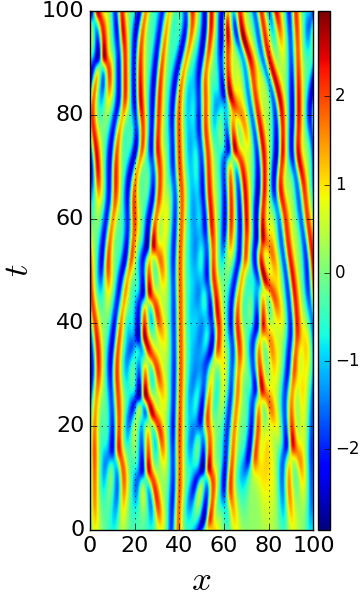
\includegraphics[height=0.35\textheight]{KS_L100N256}
  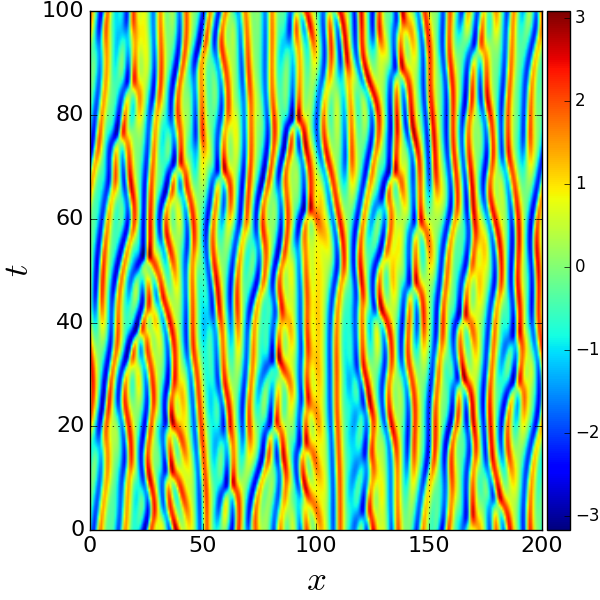
\includegraphics[height=0.35\textheight]{KS_L200N256}
  \caption[\Spt\ plots of the one\dmn\ \KSe\ for $L=100$ and $200$.]{
    Simulations of the one\dmn\ \KSe\ for domain size $L=100, 200$ respectively with random initial
    conditions. The color represents the magnitude of $u(x, t)$.
  }
  \label{fig:KS_L100200}
\end{figure}

To summarize, the form of the \KSe\ \refeq{eq:ks} on a periodic domain in one
space dimension that we use in this report is
\beq
    u_\zeit =  - u u_\conf
    -u_{\conf \conf}-u_{\conf \conf \conf \conf}
\,,\qquad
    x\in [0,L]
\,,
\ee{ACe-ks}
where subscripts denote partial derivatives.

\section{Numerical setup}
\label{sect:KSnumer}
	\input{../chen/projectFall17/chapters/KSnumerical}

\section{Symmetries of \KSe}
\label{sect:KSsym}
    \section{Symmetries}
\label{sect:kssym}

The one\dmn\ \KSe\ has three different
symmetries. Suppose $u(x, t)$ is an orbit in this system, then we have
\begin{itemize}
\item \emph{Galilean invariance}: $u(x-ct,t)+c$ is also a
  valid orbit, where c is a constant
  number. These two orbits have different mean velocity
  $\int dx\, u$.
\item \emph{Reflection invariance}:   $-u(-x,t)$ is also a valid orbit.
  In the Fourier mode space, reflection takes form $a_k \to -a_k^{*}$.
\item \emph{Translation invariance}: $u(x+\ell,t)$ is another valid orbit.
  In the Fourier mode space, translation takes form $a_k \to e^{iq_k\gSpace} a_k$
  with $\gSpace = 2\pi \ell/L$.
\end{itemize}
The zeroth Fourier mode $a_{0}$ represents the
mean velocity of $u(x, t)$. by setting $a_{0}=0$ in the integrator,
we eliminate the Galilean symmetry.
Therefore, we only need to account for the \On{2} symmetry of this system.
Reflection in \statesp\ \eqref{eq:fourierspace} takes the form
\[
  R=\diag(-1,\, 1, \, -1, \, 1,\cdots)
  \,.
\]
The translation symmetry corresponds to an one-parameter \SOn{2}
group in the \statesp,
\[
  \LieEl(\gSpace)=\diag(r_{1},r_{2},\cdots,r_{N/2-1})
\]
with
\[
  r_{k}=
  \begin{pmatrix}
    \cos k\gSpace & \sin k\gSpace \\
    -\sin k\gSpace & \cos k\gSpace
  \end{pmatrix}
  %,\quad k=1,2,\cdots,N/2-1
  \,.
\]
The corresponding Lie group generator is
\[
  \Lg= \diag(t_{1},t_{2},\cdots,t_{N/2-1}),\quad
  t_{k}=
  \begin{pmatrix}
    0 & k \\
    -k & 0
  \end{pmatrix}
  \,.
\]
Based on the consideration of these symmetries,
there are three types of invariant orbits in \KS\ system: \po s in the
$b_k=0$ invariant antisymmetric subspace, pre\po s which are self-dual
under reflection,
and \rpo s with a shift along group orbit after one
period. As claimed in \refref{SCD07}, the first type is absent for a domain
as small as $L=22$, and thus we focus on the last two types of orbits.
\begin{itemize}
\item
  For pre\po s $\cssp(0)=R\cssp(\period{p})$ , we only need to evolve
  the system for a prime period $\period{p}$ which is half of the whole
  period. The Floquet matrix is
  $\jMps_{p}(\cssp)=R\jMps^{\period{p}}(\cssp)$.
\item
  A \rpo,
  $\cssp(0)=\LieEl_p\cssp(\period{p})$, returns after one period
  $\period{p}$ to the initial state upon the group transform
  $\LieEl_p=\LieEl(\gSpace_p)$, so the corresponding Floquet matrix is
  $\jMps_p(\cssp)=\LieEl_p\jMps^{\period{p}}(\cssp)$.
\end{itemize}
In later sections, we calculate the stability of both pre\po s
and \rpo s. We anticipate that there are two marginal directions
for both types of orbits. One marginal direction corresponds to the
velocity field and the other one is the group tangent, which is
proved in \refexam{exam:KSmarginal}.
%%%%% example start %%%%%
\exampl{
  $\vel(\cssp)$ and $\groupTan(\cssp)$ are the two marginal directions
  of both pre\po s and \rpo s}{
  \label{exam:KSmarginal}
  The \JacobianM\ transports both velocity field and group tangent along the
  flow $\jMps^{\period{p}}\vel(\cssp(0)) = \vel(\cssp(\period{p}))$,
  $\jMps^{\period{p}}\groupTan(\cssp(0)) = \groupTan(\cssp(\period{p}))$.
  Therefore, for pre\po s, we have
  $\jMps_p\vel(\cssp(0)) = R\vel(\cssp(\period{p}))
  =R\vel(R\cssp(0))$.
  Here, we have used the definition of a pre\po\ and the form of
  its Floquet matrix. By use of the equivariance relation of
  the velocity field
  under reflection $\vel(R\cssp(0)) = R\vel(\cssp(0))$, we get
  \[
    \jMps_p\vel(\cssp(0)) = R \cdot R\vel(\cssp(0)) = \vel(\cssp(0))
    \,.
  \]
  So, we see that the velocity field is one marginal direction of pre\po s
  with Floquet multiplier $1$. Similarly, for the group tangent we have
  $\jMps_p\groupTan(\cssp(0)) = R\groupTan(R \cssp(0)) =
  R \cdot \Lg \cdot R \cssp(0) $ following definition \refeq{eq:gTan}.
  Since reflection anti-commutes with rotation $R\Lg + \Lg R = 0$, then
  we have
  \[
    \jMps_p\groupTan(\cssp(0)) = -\Lg \cdot R \cdot R \cssp(0) =
    -\groupTan(\cssp(0))
    \,.
  \]
  Therefore, the group tangent is also a marginal direction of pre\po s
  but with Floquet multiplier $-1$.  A group tangent reverses direction
  after one period for pre\po s.


  For \rpo s, by a similar process we have
  \[
    \jMps_p\vel(\cssp(0)) = \LieEl_p \vel( \LieEl_p^{-1} \cssp(0)) = \vel(\cssp(0))
  \]
  and
  \[
    \jMps_p\groupTan(\cssp(0)) = \LieEl_p \groupTan( \LieEl_p^{-1} \cssp(0))
    = \groupTan(\cssp(0))
    \,.
  \]
  So, the velocity field $\vel(\cssp)$ and the group tangent  $\groupTan(\cssp)$
  are two degenerate \Fv s for \rpo s, but not degenerate for
  pre\po s.
}
%%%%% example end %%%%%
In order to reduce \On{2} symmetry, we can choose to
reduce reflection symmetry first and then translation
symmetry, or vice versa.
Note that reflection does not commute with translation
$R\LieEl(\gSpace) = \LieEl(-\gSpace)R$,
so the result of symmetry reduction depends on the order
we choose.
In this section, we elect to quotient out the \SOn{2} symmetry
by the technique described in \refsect{sec:symReduce},
more precisely, by the 1st mode slice\rf{BudCvi14}
defined by
\begin{equation}
  \label{eq:ksslice}
  c_1 = 0 ,\, b_1 >0
  \,.
\end{equation}
This corresponds to choosing
$\slicep = (1, 0,\cdots, 0)$ as the template point
in \refeq{eq:slice}.
The reduced \statesp\ is denoted as
\begin{equation}
  \label{eq:KSspred}
  \sspRed=(\hat{b}_{1}, \hat{b}_{2}, \hat{c}_{2},\cdots, \hat{b}_{N/2-1}, \hat{c}_{N/2-1})^\top
  \,.
\end{equation}
Here, $\hat{c}_{1} = 0$ is omitted explicitly.
We can rotate orbits in the full \statesp\ to
the \SOn{2}-reduced \statesp\ by transformation
$a_k \to e^{-ik\gSpace_1}a_k$ where $\gSpace_1$ is the phase of the first Fourier mode.
Alternatively, we can choose to integrate the system directly in the slice.
For a reduced \statesp\ point \refeq{eq:KSspred}, which is
a $(N-3)$-element vector, the corresponding group tangent in the full
\statesp\ is
$\groupTan(\sspRed) = (0, -\hat{b}_{1}, 2\hat{c}_{2}, -2\hat{b}_{2}, \cdots,
(N/2-1)\hat{c}_{N/2-1}, -(N/2-1)\hat{b}_{N/2-1})^\top$.
The template point is $\slicep=(1,0,\cdots,0)$;
then the corresponding group tangent is $\sliceTan{} = (0, -1, 0, \cdots, 0)$.
From \refeq{MFdtheta}
we get the dynamics in the slice
\[
  \velRed(\sspRed) = \vel(\sspRed)
  \,-\, \dot{\gSpace}(\sspRed) \groupTan(\sspRed)
  \,,\quad
  \dot{\gSpace}(\sspRed) = \frac{-\Im[\vel_1(\sspRed)] }{ \hat{b}_{1} }
  \,.
\]
When an in-slice orbit gets close to the slice border $\hat{b}_1 = 0$,
the trajectory can attain arbitrarily high speed.
To alleviate this numerical difficulty,
we rescale the time step by $dt=\hat{b}_1 d\tau$.
Thus the time-rescaled dynamics in the slice is
\begin{equation}
  \label{eq:ksRescale}
  \frac{d \sspRed}{d\tau} = \hat{b}_1 v(\sspRed) + \mathtt{Im}[v_1(\sspRed)] t(\sspRed)
  \,.
\end{equation}


\section{\KS\ on a spatial strip}
\label{ACsect:KStimeInt}
    % siminos/gudorf/thesis/chapter/KStimeInt.tex
% $Author: predrag $ $Date: 2020-05-25 15:18:45 -0400 (Mon, 25 May 2020) $

%\section{Spatially periodic \KS}
%\label{sect:KStimeInt}

%    \PCedit{
%[{\bf 2016-02-06 Predrag}
%summarize the standard case on spatially $\speriod{}$-periodic domain]
%    }

It is not possible to integrate numerically the \KSe\ on the
\spt ly doubly infinite domain \refeq{e-ks}. Instead, the standard practice
is to confine the system to a spatially \speriod{}-periodic domain,
specify a smooth spatially periodic initial condition
$u(\conf,\zeit)=u(\conf+\speriod{},\zeit)$, and integrate
\beq
    u_\zeit + u_{\conf \conf} + u_{\conf \conf \conf \conf} + u_\conf u = 0
    \,,\quad
    x \in [0,\speriod{})
    \label{e-ksL}
\eeq
forward in time on the \spt\ cylinder of  \reffig{fig:spaceTime1}\,(a).
Though stable periodic solutions do exist\rf{FSTks86}, for a  generic,
sufficiently
large spatial domains, all numerical \KS\ solutions exhibit ``steady
state turbulence'' illustrated by \reffig{f:ks_largeL}.

%%%%%%%%%%%%%%%%%%%%%%%%%%%%%%%%%%%%%%%%%%%%%%%%%%%%%%
\begin{figure}[h]
    \begin{center}
\begin{minipage}[height=.20\textheight]{.18\textwidth}
\centering
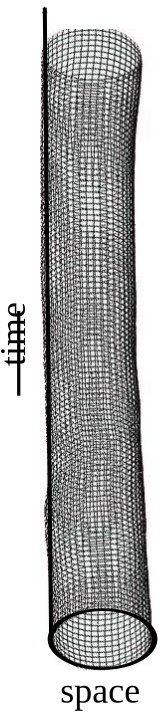
\includegraphics[width=.75\textwidth]{cylinderTime1}
    \vfill
\small{\texttt{(a)}}
\end{minipage}
~~~~
\begin{minipage}[height=.20\textheight]{.75\textwidth}
\centering
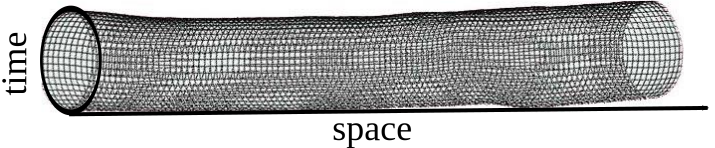
\includegraphics[width=.80\textwidth]{cylinderSpace1}
\\
\small{\texttt{(b)}}
\\
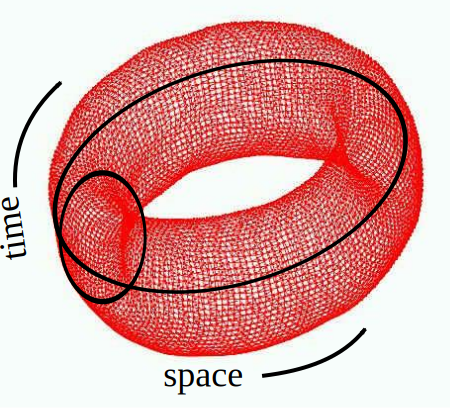
\includegraphics[width=.50\textwidth]{spaceTime1}
\\
\small{\texttt{(c)}}
\end{minipage}
    \end{center}
\caption{\label{fig:spaceTime1}
(a) The 1D \KSe\ is usually integrated on a \spt\ cylinder of an
    arbitrary fixed $\speriod{}$ periodic spatial extent, with time
    $\zeit\in\{-\infty,\infty)$; for an example, see \reffig{f:ks_largeL}.
(b) It is also possible to integrate the equation on a \spt\ cylinder of an
    arbitrary fixed $\period{}$ periodic temporal extent, with position
    ranging over $\conf\in\{-\infty,\infty)$, see \refsect{sect:KSspaceInt}.
(c) Here we shall seek {\spt}ly \twot\ solutions $u(\conf,\zeit)$ over a 2-torus of
    dynamically determined size $(\speriod{},\period{})$ , see
    \refsect{sect:KStwots}.
}
\end{figure}
%%%%%%%%%%%%%%%%%%%%%%%%%%%%%%%%%%%%%%%%%%%%%%%%%%%%%%


Smooth, spatially periodic velocity field $u$ %(\conf,\zeit)=u(x+\speriod{},\zeit)$
is naturally represented in the Fourier space,
\beq
  u(\conf,\zeit)
   =\sum_{m=-\infty}^{+\infty} a_m(\zeit)\,e^{ i 2\pi m\conf /\speriod{} }
\,,
\ee{eq:ksexp}
with the $1$D PDE \refeq{e-ksL}
replaced by an infinite set of
ODEs for the complex Fourier coefficients $a_m(t)$:
\beq
\dot{a}_m %= \pVeloc_m(a)
     = ( q_m^2 - q_m^4 )\, a_m
    - i \frac{q_m}{2} \sum_{k=-\infty}^{+\infty} a_k a_{m-k}
\ee{SCD07:expan}
where $q_m =  2\pi m/\speriod{}$.
Since $u(\conf,\zeit)$ is real, $a_m=a_{-mm}^\ast$, and we can replace the
sum by a $m > 0$ sum.


Consider the \KSe\ \refeq{e-ks} on a {\spt} cylinder
$(\conf,\zeit)\in([0,\speriod{}),\reals)$, defined on a a spatial strip of width
$\speriod{}$, with spatially periodic boundary condition $u(\conf,\zeit)=u(x+\speriod{},t)$, see
\reffig{fig:spaceTime1}\,(a).
Discretize spatially the \KS\ system by Fourier expanding the field
$u(\conf_n,\zeit)= u_n(\zeit)$ over $N$ points of a periodic spatial 1D
lattice $\conf_n=n\speriod{}/N$,
\bea
  \Fu_k(\zeit) &=& \frac{1}{N} \sum^{N-1}_0 u_n(\zeit) e^{-iq_k\conf_n}
  \,=\, \frac{1}{N} \sum^{N-1}_0 u_n(\zeit) e^{-i 2 \pi k n /N}
  \,,\quad
q_k = \frac{2 \pi k}{\speriod{}}
\continue
  u_n(\zeit) &=&\sum_{k=0}^{N-1}\Fu_k(\zeit) e^{iq_k\conf_n}
    \,=\, \sum_{k=0}^{N-1}\Fu_k(\zeit) e^{i 2 \pi k n /N}
\,,
\label{spatFT}
\eea
and expressing \refeq{e-ks} in terms of discrete spatial Fourier modes as
$N$ ordinary differential equations (ODEs) in time
\beq
%\dot{\Fu}_k(\zeit)
\frac{d~}{d\zeit}\Fu_k(\zeit)
= ( q_k^2 - q_k^4 )\, \Fu_k(\zeit)
- \frac{i q_k}{2} \!\sum_{k'=0}^{N-1} \!\!\Fu_{k'}(\zeit) \Fu_{k-k'}(\zeit)
\,.
\label{e-Fks}
\eeq

        \PCedit{
In the Fourier representation the \reqva\ time dependence is
\beq
 a_k(t) e^{-itc q_k} = a_k(0)
\,.
\ee{reqvaF}
Differentiating with respect to time, we obtain
the Fourier space version of the \reqv\ condition
\refeq{KSeqvCond},
\beq
 \pVeloc_k(a) - i q_k c a_k = 0
\,,
\ee{reqvCondF}
which we solve for (time independent) $a_k$ and $c$.
        }


%%%%%%%%%%%%%%%%%%%%%%%%%%%%%%%%%%%%%%%%%%%%%%%%%%%%%%%%%%%%%%%%%%
\subsubsection{Temporal stability}
\label{exam:KurSivTempstab}
% From ChaosBook Chapter{PDEs}{2016-01-23}{Turbulence?}

To calculate the temporal stability of a spatial \eqv\ $\Fu_\stagn$
    \PC{2019-05-16}{dropped
(or a temporally \po).
%\refeq{eq:StabMat} is plain wrong, no?
    }
we need to evaluate  the \stabmat\ (the matrix of temporal
velocity gradients)
\beq
%  \Mvar_{ij}(a_q)  = \left.\frac{\partial v_i}{\partial a_j}\right|_{a=a_q}
  \Mvar_{ij}(\Fu_\stagn)  =
  \left.\frac{\partial \dot{\Fu}_i}{\partial \Fu_j}\right|_{\Fu={\Fu_\stagn}}
\,.
\label{eq:StabMat}
\eeq
For \KS\ we can
compute $\Mvar(\Fu_q)$ efficiently using the linearity
of the Fourier transform, see \refref{SCD07}.
Consider the four matrices
$\frac{\partial \dot{b}_k}{\partial b_j},\frac{\partial
\dot{b}_k}{\partial c_j},\frac{\partial \dot{c}_k}{\partial
b_j},\frac{\partial \dot{c}_k}{\partial c_j}$,
where the real and imaginary parts of $\Fu_k$ are
$\Fu_k=b_k+ic_k$.
For illustration, consider the $b_k=0$ invariant antisymmetric subspace
$\bbU^+$,
\beq
\dot{c}_k= \pVeloc_k(c)
     = ( q_k^2 - q_k^4 )\, a_k
    - \frac{q_k}{2} \sum_{m=-\infty}^{\infty} c_m c_{k-m}
\,,\qquad   q_k = k/2\pi \speriod{}
\,.
\ee{expan}
The temporal {\stabmat} \refeq{eq:StabMat} restricted to the invariant
antisymmetric subspace $\bbU^+$ follows from \refeq{expan}:
\beq
{\Mvar}_{kj}(c) =\frac{\pde v_k(a)}{\pde c_j  }
=(q_k^2- q_k^4)\delta_{kj} + q_k ( c_{k-j}- c_{k+j})
\,.
\ee{expanMvar}
For the full \statesp, consult sect.~6.2 {\em Calculating stability of equilibria}
of Siminos thesis\rf{SiminosThesis}.

\subsubsection{\KS\ $u=0$ temporal equilibrium}
\label{sect:KSu0equiT}

The \KS\ flat flame front $u(\conf,\zeit)=0$ is always a temporal {\eqv} of \refeq{e-ks},
whose temporal {\stabmat} \refeq{expan} is
diagonal, with real temporal stability exponents $\eigExp[k]= q_k^2- q_k^4$,
the eigenvectors are spatial Fourier modes, and consequently the
temporal {\jacobianM} is diagonal as well,
\(
\jMps^t_{kj} = \delta_{kj} \ExpaEig_k(\zeit)
    \,,\;
\ExpaEig_k(\zeit) = e^{(q_k^2- q_k^4)\,t}
\,.
\)
%	} %end \example{\Stabmat,  antisymme
%%%%%%%%%%%%%%%%%%%%%%%%%%%%%%%%%%%%%%%%%%%%%%%%%%%%%%%%%%%%%%%%%%


\section{Michelson method applied to \KSe}
\label{chap:KSmichelson}
    \input{../chen/projectFall17/chapters/KSmichelson}

\section{Yang method applied to \KSe}
\label{chap:KSyang}
    \input{../chen/projectFall17/chapters/KSyang}

\section{Summary}
\label{sect:summary}
    %  conclusion.tex
% $Author: predrag $ $Date: 2009-08-20 12:41:28 -0400 (Thu, 20 Aug 2009) $

\section{\Statesp\ geometry of spatially extended systems}


This thesis contribution to the dynamical system's approach
to spatially extended systems is to provide a framework for
elucidating state space geometry in the presence of
continuous symmetries. The presence of symmetry enriches
\statesp\ structure and profoundly influences dynamical
behavior. A a striking example is provided by the robust
homoclinic (or heteroclinic) connections in \KS\ flow
(discussed in \refchap{chap:kseStSp}) that provide a
recurrence mechanism by connecting neighborhoods of saddles
along a homoclinic (or heteroclinic) loop and organizing a
group of {\rpo s} around them.

The  \statesp\ structure remains unclear until points related
by continuous symmetry are identified and the dynamics is visualized in
reduced \statesp. Once this reduction procedure was carried out for \KS\ flow
we were able to identify (in \refchap{chap:kseRedStSp}) the
``stretching and folding'' of the unstable manifold of a \reqv\ as
the mechanism responsible for organizing a different group of \rpo s. Moreover
we were able to demonstrate that \rpo s  follow the unstable manifold of \REQV{\pm}{1}
for a while until carried over to the unstable manifold of \EQV{2} therefore
revealing the interplay of unstable manifolds of different objects, living
in subspaces with different symmetry, in shaping the geometry of the attractor.

The understanding of the geometry of \KSe\ for $L=22$ is by
no means complete. The obvious next step is to identify
suitable Poincar\'e sections for the study of unstable
manifolds and the \rpo s clustered around them. Contrary to
the \CLe\ example of \refchap{chap:lasers} where a global
section was found and the dynamics was described as a first
return map to the section, in the case of \KS\ equation we
will need more than one sections. Each section will be used
to capture the dynamics of the unstable manifold of a
(relative) equilibrium until it starts folding back to
itself. Parameterizing the intersection of a manifold with
the \Poincare\ section by Euclidean length along it, a
forward map from section to section will be constructed and
convolution of those maps will result in a return map. This
approach meshes very well with the construction of a Markov
partition of the dynamics, if such a partition is within
reach. A potential obstacle is that unstable manifolds of
objects of interest for \KS\ dynamics are often
high-dimensional, \eg $4$-dimensional for \REQV{\pm}{1}, and
their visualization and parametrization is a non trivial
task. Nevertheless, since the separation of the leading
eigenvalues is large, we expect that the continuation of the
strongly unstable eigenspace will play the dominant role.
Furthermore, we still need to investigate the role played by
trajectories originating in the $\eigExp[1,2]$ eigenspace of
\EQV{1} that are not in the antisymmetric subspace and are
therefore expected to play a role in organizing the
relative periodic orbits.


\section{Symmetry reduction}

For this geometric understanding to be possible we had to develop a
a symmetry reduction procedure for our specific needs
and with the following
constraints in mind:
1) the method must work efficiently in high-dimensional \statesp, 2) reduction
can be local but the local pieces have to be joined together in
a way that the global geometry of the attractor is elucidated.

For visualization purposes the method of moving frames is efficient in providing
symbolic expressions for invariants up to moderate dimension. When the
representation of the symmetry group is a direct sum of irreducible representations,
as usually is the case with discretizations of PDEs, we can define a moving
frame in one irreducible subspace and construct invariants for the rest of
the irreducible subspaces, as necessary for visualization.
The invariants thus obtained are singular but the singularities can be removed,
or merely moved away from regions of dynamical interest.
Then solutions computed in the equivariant variables can be visualized
in the invariant basis without any discontinuities introduced.

This leads us to the next step, which is reduction using the
geometrical interpretation of moving frames as a group
operation that brings points back to a local {\csection} of
group orbits. This is a linear operation for any given point
and can be implemented efficiently even for high-dimensional
discretizations of PDEs. The crucial step is to avoid
transformation singularities by restricting attention to
local, group-invariant Poincar\'e sections that do not
contain any points on which the transformations become
singular.

As noted in the introduction, a method of symmetry reduction
for PDEs has been presented by Rowley and
Marsden\rf{rowley_reconstruction_2000}, that allows one to
integrate a PDE defined in the reduced space along with a
reconstruction equation to recover the dynamics of the
original problem. This procedure identifies the reduced space
$\Manif/\Group$ with a subset of $\Manif$, called a slice, in
the same spirit we identified the reduced space with a
cross-section.
    \PC{rewrite this sentence}
The reconstruction equation is guaranteed to
work locally, in the neighborhood of the initial condition
but can fail globally. In \refref{rowley_reconstruction_2000}
choosing a new slice is proposed as a method to overcome this
difficulty and the different slices are to be treated as
local coordinate charts on $\Manif/\Group$. Yet, this can
obscure the study of global aspects of dynamics. It will be
interesting to investigate how this difficulty is connected
to the singularities present in the moving frame method and
whether the insight gained here can help one avoid
singularities while still identifying the reduced space with
a single slice.


    \PC{
perhaps mention as future generalizations: invariant tori -
``larger'' symmetries?
    }


\renewcommand{\cl}[1]{{\ensuremath{|#1|}}}  % the length of a periodic orbit, Ronnie

%%%%%%%%%%%%%%%%%%%%%%%%%%%%%%%%%%%%%%%%%%%%%%%%%%%%%%%%%%%%%%%%%%%%%%%
\printbibliography[heading=subbibintoc,title={References}]
